\documentclass{article}
\usepackage{handout}
\usepackage{algorithm}
\usepackage{myhyperlinks}
\usepackage{graphicx}

%\newcommand{\cmt}[1]{\textsf{[#1]}}

\begin{document}

\title{Galant: A Graph Algorithm Animation Tool\thanks{
    This work is the result of a senior design project at North Carolina
    State University, Department of Computer Science.
    The first author conceived and guided the project while the others
    provided the implementation details.
    We thank Dr. Robert Fornaro and Margaret Heil, the instructors, for
    coordinating the project(s) and providing instruction in communication
    skills, respectively. Ignacio Dominguez provided valuable technical
    support.
    An alpha testing version of the software is available on request.
    %% provided the recipient (i)~gives a report on how it was used;
    %% and (ii) gives us feedback on features that were desirable, additional
    %% features that would make Galant more useful, bugs, and annoyances.
  }
}
\author{Matthias Stallmann\thanks{Matthias Stallmann, Department of Computer
    Science, North Carolina State University, Raleigh NC, 29695-8206.
    email: \texttt{mfms@ncsu.edu}}
  \and Jason Cockrell
  \and Tynan Devries\thanks{SAS Institute, Cary NC.}
  \and Alexander McCabe\thanks{Elsinore Technologies, Raleigh NC.}
  \and Michael Owoc\thanks{IBM, Durham NC.}
}

\maketitle

\begin{abstract}

  A host of algorithm animation programs have been developed over the
  years. Primarily these have been designed for classroom use and involve
  considerable overhead for the animator of the animations (an instructor or
  developer) --- students are passive observers.  We distinguish three
  primary roles: the \emph{observer}, who simply watches an animation; the
  \emph{explorer}, who is able to manipulate problem instances; and the
  \emph{animator}, who designs an animation.  A key feature of Galant\footnote{
    Aside from being an acronym, Galant is a term for a musical style
that featured a return to classical simplicity after the complexity of the late Baroque era. We hope to achieve the same in our approach to algorithm animation.
} is that
  it simplifies the role of the animator so that students can create their
  own animations by adding a few visualization directives to pseudocode-like
  implementations of algorithms.  The focus on graph algorithms has a key
  advantages: the objects manipulated in an animation all have the same
  type.
  The restrictions to graphs need not be a limitation:
  graphs are ubiquitous and Galant therefore provides a framework for
  animations in domains beyond classic graph algorithms; examples include
  search trees, automata, and even sorting.

  Galant is also distinguished in that it is a tool rather than a closed
  system.  In other words, it is designed to interact easily with other
  software such as text editors, other graph editors, other algorithm
  animation tools, graph generators, Java API's, format translation filters
  and graph drawing programs. This interactivity significantly expands the
  range of Galant's applications, including, for example, as a research tool
  for exploring graph algorithms.


\end{abstract}

\section{Background}

Algorithm animation has a long history, dating back at least as far as the
work of Brown and Sedgewick~\cite{1988-Computer-Brown,1985-IEEE_Software-Brown}
and that of Bentley and Kernighan~\cite{1987-Animation-Bentley} in the 1980's.
The BALSA software, developed by Brown and Sedgewick, is a sophisticated system that provides several
elaborate examples of animations, including various balanced search trees,
Huffman trees, depth-first search, Dijkstra's algorithm and transitive closure.
The Bentley-Kernighan approach is simpler: an implementation of an algorithm is annotated with output directives that trace its execution.
These directives are later processed by an interpreter that
converts each directive into a still picture (or modification of a previous
picture). The pictures are then composed into a sequence that is navigated by the user.

In discussing algorithm animation software,
we distinguish three primary roles: the \emph{observer}, who simply
watches an animation; the \emph{explorer}, who interacts with an animation by,
for example, changing the problem instance (graph); and the \emph{animator}, who
designs an animation. The latter may also be referred to as a
\emph{developer} if the process of creating animations is integrated with
that of implementing the animation system.\footnote{
  With Galant a \emph{developer} is someone who participates in modifying the
  underlying Galant implementation, an activity completely independent of creating
  animations.
}
An explorer needs to be an observer as well
and an animator needs to be both of
the others.
R\"ossling and Freisleben~\cite{2002-JVLC-Roessling} articulate a similar
classification of roles.

We also define an algorithm animation \emph{tool} as animation software specifically designed to interact easily with other programs such as
text editors, other graph editors, other algorithm animation tools,
graph generators, Java API's, format translation filters and
graph drawing programs.

A hypothesis, at least partially validated (using student attitude
surveys~\cite{1997-SIGCSE-Stasko}) is
\begin{enumerate}
  \item \label{item:demonstration}
    The value added --- beyond lectures and textbook
    --- for students watching an animation (observer role)
    is minimal.
  \item \label{item:interactive}
    If students are able to manipulate problem instances (explorer role)
    the gain is more significant.
  \item \label{item:creative}
    Students who implement algorithms and design simple animations of them
    (animator role) are likely internalize the structure of the algorithm and
    come away with significant understanding of it.
\end{enumerate}

We call animations that are designed for (\ref{item:demonstration}) above, i.e., observer focused,
\emph{demonstration} animations;
those designed for (\ref{item:interactive}), i.e., for both observer and explorer, are
\emph{interactive} animations; those designed for (\ref{item:creative}) are
\emph{creative} animations.

% A hypothesis, at least partially validated (using student attitude
% surveys~\cite{1997-SIGCSE-Stasko}) posits that,
% while students acting as observers or explorers of animations may gain some benefit,
% a student who takes on the role of animator has a much richer learning
% experience.
% This hypothesis has become Galant's major motivating factor --- that it should
% simplify the task of the animator as much as possible while enhancing
% the ability to produce compelling animations.

% [Last modified: 2013 06 26 at 18:44:29 GMT]


\section{Related work}

There is a large variety of algorithm animations available. Here we focus solely on those that offer significant mechanisms for creating new animations.
These differ primarily in (i)~the role of the user (primarily observer
or explorer as well); and
(ii)~the challenges imposed on the animator.
Almost all of these are systems rather than tools.
For a comprehensive survey of graph algorithm animation and graph drawing
as educational tools see Bridgeman~\cite{2013-GDBook-Bridgeman}. 

\textbf{Observer-oriented (passive) systems.}
One general purpose animation program is ANIMAL~\cite{2002-JVLC-Roessling,ANIMAL};
it provides the animator
with a rich menu
of elements common to many algorithms.
Steps in the animation are linked to steps in the pseudocode.
Though there are many options for creating interesting animations,
it appears that these are passive.

Galles~\cite{Galles} is an animation tool with very
sophisticated creation options.
Primarily designed to be passive, it could conceivably, with a parser
for a graph input format and a mechanism that allows the user to view and
manipulate the input graph, be made interactive.
Then it would also be a tool.
It suffers, however, from the fact that the
animator must navigate a complex Java-based interface.

Although secondary to its main purpose as a library of data structures and
algorithms,
LEDA~\cite{1999-LEDA-Mehlhorn} offers a graph window facility that can be
used to create animations of graph algorithms.
The documentation gives several examples and illustrates the rich functionality of
the drawing and visualization capability of graph windows.
Since LEDA is a general purpose, C++-based, programming language for
algorithms and data structures, it is easily augmented with extensions that
are integrated seamlessly with the core API; in this case, graph windows work
in concert with core graph functions and macros.
%%  (which are similar to, but
%% more sophisticated than, those in GDR).
Unfortunately LEDA is a commercial product with
non-trivial licensing cost.

\textbf{Explorer-oriented (interactive) systems.}
Several online applets feature graph algorithm animation. Of these,
JAVENGA~\cite{JAVENGA} stands out. It is highly interactive. The drawing and
editing of
graphs is simple and intuitive, and graphs can be viewed in all three major
representations (drawing, adjacency matrix and adjacency list).
The variety of graph algorithms available is impressive:
breadth-first and depth-first search, topological sort, strongly connected
components, four shortest path algorithms, two minimum spanning tree
algorithms, and a network flow algorithm.
Animations can be run one step at a time with the option of moving backwards
or continuously with an adjustable number of milliseconds per step.
Javenga's main drawback is that the explorer is unable to save graphs for
future sessions.

The j-Alg~\cite{j-Algo} is an impressive animation system.
It is highly interactive, has a relatively easy to use interface, and has sophisticated animations for a large variety of algorithms,
including graph searching, Dijkstra's algorithm,
algebraic path problems (generalizations of all-pairs shortest paths and transitive closure), AVL trees, Knuth-Morris-Pratt string searching and BNF syntax diagrams.
Its only drawback is that there is no readily available mechanism
for outsiders to create new animations.
New animations are developer-created and released periodically.

\textbf{Animator-oriented systems.}
Edgy~\cite{Edgy} is nn applet that combines exploration, simple programming techniques
(using the Snap~\cite{Snap} language) and a simple graph API.
Since it stores graphs in \texttt{dot} format -- see~\cite{GraphViz} --
and programs in \texttt{xml},
it could be expanded into a tool akin to Galant.
However, the programming capabilities are primitive;
it would be difficult, for example, to add sophisticated data structures such as
priority queues or external Java API's.
From the tutorial videos for Edgy it is clear that the software is designed
for users who are just learning to program.

\textbf{Libraries.}
AlgoViz~\cite{AlgoViz}
is a large catalog of algorithm animations, continually updated by
contributors who either submit new animations or comment on existing ones.
Like any large repository with many contributors, AlgoViz is difficult to
monitor and
maintain.
The OpenDSA project~\cite{%
2011-ProgramVisualization-Shaffer,2011-Koli-Shaffer,2012-SIGCSE-Fouh%
}
aims to create a textbook compilation of a variety of
visualizations, mostly designed for observers.

\textbf{Early work.}
Earlier animation tools/systems include GDR~\cite{1992-CSDM-Stallmann}, John Stasko's
Tango~\cite{1990-Computer-Stasko}, Xtango,
and SAMBA,\footnote{
These and Stasko's other animation tools are posted at
http://www.cc.gatech.edu/gvu/ii/softvis/
} and, of course,
the work of
Brown and Sedgewick~\cite{1988-Computer-Brown,1985-IEEE_Software-Brown}
and that of Bentley and Kernighan~\cite{1987-Animation-Bentley}.
SAMBA, and to a lesser extent GDR, is especially notable for emphasis on simplifying the creation of
animations so that students can easily accomplish them.
Both are also tools by our definition.
All of these suffer, however, from using old technology,
and, except for GDR,
they require off-line creation
of problem instances and have no graph-algorithm specific implementations
or graph creation interfaces to offer.

% [Last modified: 2013 06 26 at 18:34:44 GMT]


Galant is based on GDR, which we discuss in Section~\ref{sec:gdr_features}.
We then give an overview of Galant -- Section~\ref{sec:galant_overview}.
The most important aspect of Galant is the ability to create animations easily,
as discussed in Section~\ref{sec:animator}.
Then we give a brief overview of the user interface --
Section~\ref{sec:user_interface}; a more detailed description is given in Appendix~\ref{sec:user_documentation}.

\subsection{GDR: Galant's predecessor}
\label{sec:gdr_features}
Galant is a successor to
GDR~\cite{1991-TR_NCSU_CSC-Stallmann,1992-CSDM-Stallmann} and has much of the
same functionality.
The design of GDR is illustrated in Fig.~\ref{fig:gdr}.
To the left of the dotted line are the interactions with external entities,
as supported by GDR.
The GDR user, when running a specific animation created and compiled
externally, acts as both the editor of problem instances and as initiator of an
algorithm animation with which (s)he may then interact, i.e., plays the role
of explorer and of observer. 
Input and output take the form of a simple text-based file format that can be
manipulated outside of GDR via text filters, graph editors, graph drawing
applications, etc. It is this external manipulation capability
that makes GDR a tool rather than a
closed system.

The animation creator writes a C program that interacts with a graph ADT
whose functions access and/or modify both the internal representation of the
graph and the user's view of it. The ADT functions can be classified into one
of three categories depending on the graph attributes accessed:
(i)~\emph{logical} attributes --- labels (and identities) of nodes and labels
and endpoints of edges; (ii)~\emph{geometric} attributes --- the positions of
nodes and labels and
inflection points of edges; and (iii)~\emph{display} attributes ---
highlighting of nodes and edges, making labels visible/invisible, etc. 

\begin{figure}

\begin{center}
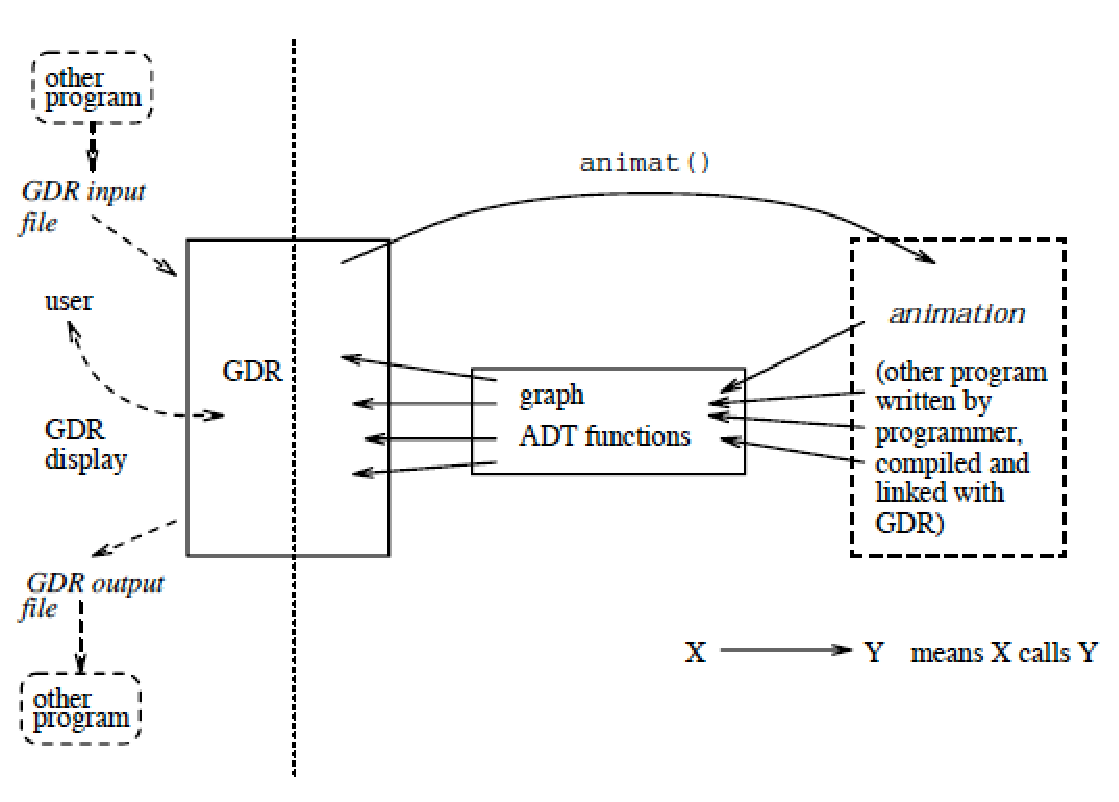
\includegraphics[scale=0.6]{X_gdr_design}
\end{center}

\caption{GDR design.}
\label{fig:gdr}
\end{figure}

While GDR has much to recommend it when compared with other algorithm
animation software, it suffers from some serious drawbacks:

\begin{itemize}
\item
  Each animation is a separate C program that interacts with an X11 window
  server.
  Therefore GDR is not portable.
  %% It is not possible to load (and apply) more than one animation to
  %% the same graph.
\item
  The user interface is crude. Aside from being black and white it has no
  file browser, no rubber-banding of moves, non-standard keyboard shortcuts
  and an unappealing look and feel.
%% \item
%%   The format for storing graphs, while simple and text-based, does not
%%   resemble any other graph format and is difficult to edit or filter.
\item
  While the API supports access to the graph itself, there is no API support for
  data structures commonly used in graph algorithms (stacks, queues, priority
  queues).
\end{itemize}

% [Last modified: 2013 06 25 at 14:51:36 GMT]


\begin{figure}[p]

\begin{center}
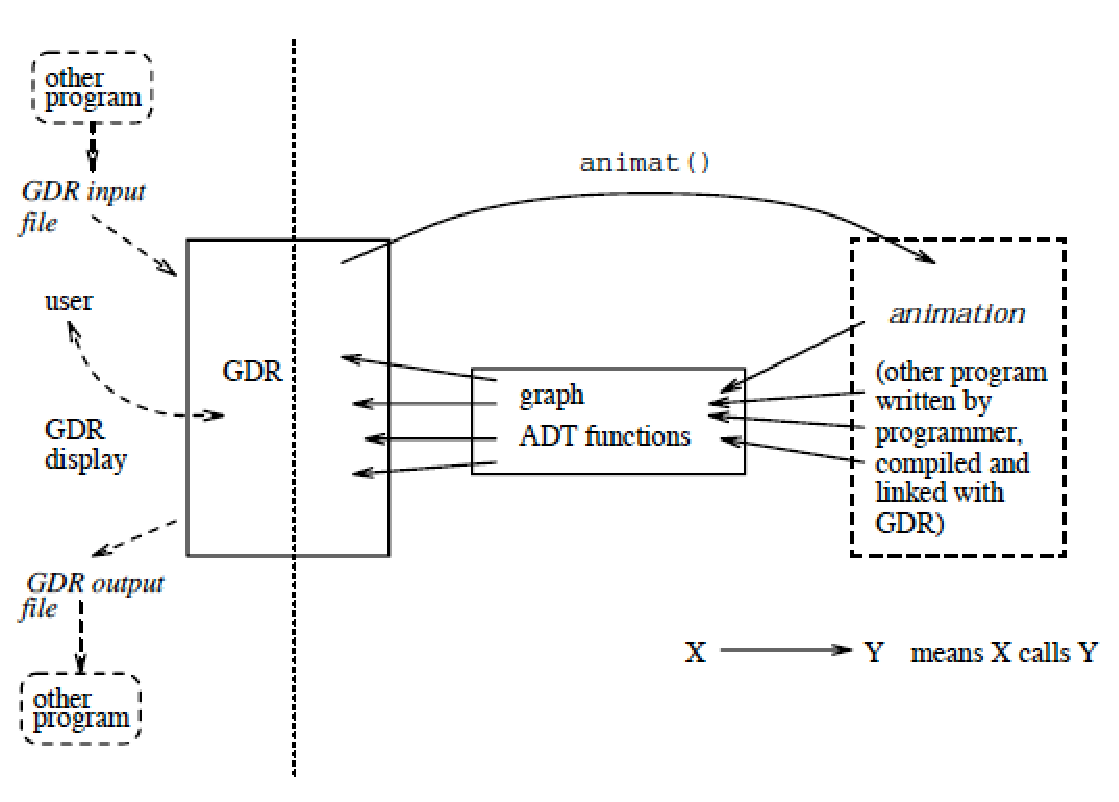
\includegraphics[scale=0.6]{X_gdr_design}
\end{center}

\caption{GDR design.}
\label{fig:gdr}
\end{figure}

\begin{figure}

\centering

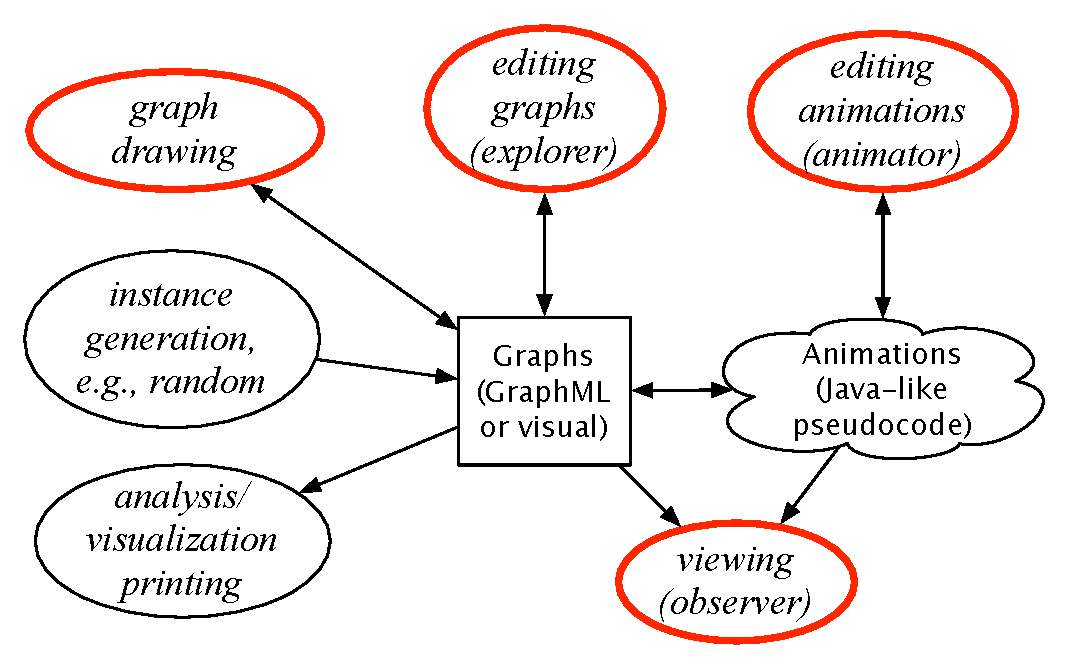
\includegraphics[width=\columnwidth]{X_overview_diagram}

\caption{Illustration of Galant design and functionality. Arrows indicate
  data flow. All functions, shown as ovals can be performed easily outside of
Galant. The ones with thick red borders are part of current Galant
functionality.}

\label{fig:overview_diagram}
\end{figure}

% [Last modified: 2013 06 25 at 16:04:45 GMT]


\subsection{Galant overview}
\label{sec:galant_overview}
Fig.~\ref{fig:overview_diagram} gives an overview of Galant functionality.
A graphical user interface (GUI) allows the user to edit both graphs and
algorithm animations, either loaded as already existing files or newly
created. At any point, the user can apply a selected animation to a selected
graph for viewing.
The animation program 
steps forward until it
displays the next animation event or, if a \texttt{beginStep()}
call has marked the start of a sequence of events, until
it reaches the next \texttt{endStep()} call.
It then pauses execution and waits for the user to decide whether to
step forward, step backward, or exit.
A step forward resumes execution while a step backward returns the display to a previous
state.
The algorithm resumes execution only when the \emph{display state}
indicated by the user's sequence of forward and backward steps
($f-b$, where $f$ is the number of forward and $b$ the number of backward steps)
exceeds the \emph{algorithm state}, the number of animation steps the algorithm
has executed.

When editing a graph the user can create/delete nodes and edges (when in the appropriate mode)
by clicking and/or
moving the mouse, and can move vertices by dragging the mouse.
There is also an interface for specifying labels, weights and colors for both
nodes and edges.
Keyboard shortcuts are available for these operations.
 
A preferences panel allows the user to select font size for labels and a
variety of other options.
Any changes to a graph are also reflected in a text (GraphML) representation
of the graph, which can also be edited directly. Naturally the GraphML
representation can also be created or edited externally: by a random or
structured graph generator, by translation from another format, by directly
editing the GraphML or by invoking a separate graph editor.
Galant has a built-in force-directed drawing program 
(see Hu~\cite{2006-Mathematica-Hu}) to position nodes
automatically if so desired.
Automatic drawing is useful when the input GraphML file does not provide position
information for the nodes (and their positions are selected randomly).
Other drawing programs, such as those provided by GraphViz~\cite{GraphViz}
and the huge body of research carried on by the graph drawing community~\cite{graph_drawing},
can be used externally as well.
Graphs used in Galant animations
can be analyzed externally using tools such as Gephi~\cite{gephi}.

Editing/compiling an algorithm animation is just like performing the same
operations on a Java program.
The compiler is essentially a Java
compiler that preprocesses the algorithm code
and compiles it, importing the relevant modules.
The preprocessor converts traversals of incidence lists and other
lists of nodes or edges into the corresponding, more obscure, Java code.
It also shields the Galant programmer from such syntactic circumlocutions
as declaring \texttt{static} methods.
Almost all Galant functions are available as both methods
using object-oriented notation, e.g., \texttt{v.highlight()},
and as procedures, e.g., \texttt{highlight(v)}.

Because the functionality of the Galant editor is limited, it is usually more
convenient to use an external program editor, reserving the Galant editor to
make minor changes in response to compile-time or runtime errors.

We use GraphML~\cite{GraphML} as our graph representation because it is
flexible, it can easily be extended, and parsers, viewers and translation
tools are becoming more common.  Because GraphML is specialized XML, parsers
for the latter, based on the Document Object Model (DOM) can be used. These
are available for many programming languages.  Translators to other formats
are also available or can easily be constructed.  For example, the
GraphViz~\cite{GraphViz} download provides one; unfortunately it preserves
only the connectivity information.  However, there is straightforward mapping
between the GraphML attributes we use (positions of nodes and colors, etc.,
of nodes and edges) and the corresponding ones in GraphViz format.  We have
written conversion scripts among the following formats: GraphML,
gml~\cite{1999-TRPassau-Himsolt}, sgf
(used for layered graphs in crossing minimization), and dot (GraphViz~\cite{GraphViz}).

% [Last modified: 2013 06 25 at 18:06:12 GMT]


\subsection{For the animator}
\label{sec:animator}
When it comes
to creating animations,
Galant offers the most significant advantages over GDR and, a fortiori,
over other algorithm animation software. Among these are:

\begin{itemize}

\item
  The API interface is simpler, due, in part, to the fact that the
  underlying language is Java rather than C.

\item
  Each node and edge has both a weight and a label. Conversion of a weight to
  a number is automatic while labels are kept as text. The programmer can
  choose the appropriate attribute, which makes the implementation more
  transparent and devoid of explicit conversions.

\item
  Most data structures are built in: stacks, queues, lists and priority
  queues of both edges and vertices. Priority queues implicitly use the
  weight attribute of the node/edge in question. The weight attribute is also
  used for sorting.

\item
  An algorithm initially designed for directed graphs can usually be applied
  to undirected graphs (and get the desired interpretation) with no change in
  the implementation.
  This is useful, for example, when implementing Dijkstra's
  algorithm.

\item
  The interface that allows an explorer to edit graph instances can also be used
  to edit, compile, and run algorithm implementations. While initial creation
  and major edits are usually more convenient via a standard program editor
  offline, an algorithm window in Galant can be used to view the algorithm and
  make corrections in response to compile or runtime errors.

\end{itemize}

The philosophy behind the API design is that it should be usable by someone
familiar with graph algorithms but only a rudimentary knowledge of Java (or
any other programming language).
The fact that Galant code resembles the pseudocode used
in one of the most
popular algorithm design and analysis texts, that of Cormen et al.~\cite{2009-Intro_to_Algorithms-Cormen},
attests to the fact that we have succeeded.

A key advantage of the API design, not present in, for example, BALSA or Edgy,
is that it sits directly on top of Java.
This allows the animator to develop arbitrarily complex algorithms using other Java class API's and ones devised by the animator.
More importantly, it allows Galant to offer significant new functionality
provided by developers with only a modicum of Java training:
\emph{sets} of nodes and edges (in addition to the stacks and queues already
built in)\footnote{
  The most recent release has sets built-in -- these were easily added by the
  developers.
}
or significant infrastructure for algorithms in a specific domain,
as was done for crossing minimization in layered graphs.


%\subsection{For the explorer}
\label{sec:explorer}

As is the case with GDR the role of observer and explorer are conflated in that
the explorer can change the graph instance via the same interface as running the
algorithm. As already pointed out, that same interface provides conveniences
to the animator as well.

\cmt{Note that the observer role differs from the explorer only in that the
  observer fails to take advantage of editing the graph, a limitation that is
  anticipated only for users not familiar with graphs; deal with this point
  under UI below?}

% [Last modified: 2013 06 04 at 19:13:02 GMT]


\subsection{The Galant user interface}
\label{sec:user_interface}
Two windows appear when Galant is started: a \emph{graph window} shows the
current graph and a \emph{text window} shows editable text.
Depending on the currently selected tab in the text window,
the text can be either a GraphML description of the current graph or an
algorithm implementation. 

The user interface is designed for all three roles.
The observer (or an instructor demonstrating an algorithm) does as follows: (a)~loads a graph using the file browser; (b)~loads an algorithm; (c)~pushes the ``Compile and Run'' button; and (d)~uses
the controls underneath the graph window or arrow keys to step through the algorithm
forward or backward as desired.

A typical explorer might edit or create a graph using the graph window and then
follow steps (b)--(d), repeating steps (a) and (d) to try out different
graphs. Saving graphs for later use is also an option.
In addition, the explorer can use the graph's tab
in the text window to fine tune the placement of
nodes or apply a force-directed graph drawing method
(as described by Hu~\cite{2006-Mathematica-Hu}) to adjust node placement.

A creator can load and edit an existing algorithm or create one from scratch
using an appropriate tab in the text window.
Compilation and execution is accomplished via the buttons at the bottom.
In fact, the code of an animation is essentially a Java program with
(a)~predefined types for nodes and edges; (b)~an
API that interacts with the graph and with intended animation effects; (c)~a
set of built-in data structures for convenience; and (d)~a set of macros that
allows the program to traverse, for example, all incident edges of a node
without invoking templated Java constructs.
Line numbers of errors reported by the compiler are those of the code
displayed in the text window.
Runtime errors are reported in the same way.
In both cases, due to the imports and macro translations, the error messages
may not be immediately intelligible, but the line numbers \emph{are}
correctly identified.

% [Last modified: 2013 06 25 at 18:08:07 GMT]


% [Last modified: 2013 06 25 at 18:08:50 GMT]


%% \section{Research applications}

%% \cmt{Illustrate use with barycenter heuristic (versus max crossings edge, if
  time permits)}

\cmt{sgf to GraphML: run heuristic, take snapshots and/or covert to dot for
  printing.}

\cmt{Another approach, from inside Galant or via a script, is to use the
  LaTeX color package in a picture environment. See, for example,\\
  http://www.ursoswald.ch/LaTeXGraphics/picture/picture.html}

% [Last modified: 2013 06 26 at 14:57:54 GMT]


\section{Future work}

Perhaps the most promising direction that our work on Galant can take is
that of developing research applications.
The benefits are twofold.
First, Galant has the potential for providing a rich environment for
the exploration of new graph algorithms or developing hypotheses about the
behavior of existing ones.
Second, as Galant is augmented with the infrastructure for specific research
domains (i.e., additional Java classes), some of the resulting functionality
will no doubt be migrated into its core. Or the core will be enhanced to
accommodate new capabilities.

One drawback of the current implementation is
that an animation runs to
completion before the user can interact with it.
This precludes certain types of interactions.
For example, one might want the user to be able to select the next node to
visit during a depth-first search or a node to insert or remove during an animation of
a binary search tree.

An algorithm implementation, despite the preprocessing we provide, still
requires some undesirable Java-specific syntax and generates highly
unfriendly error messages at both compile and runtime --- the compiler, after
preprocessing deals with raw Java code. Automatic insertion of semicolons at
the ends of lines would prevent some of the strangest error messages. There
are also serious issues with the use of global variables, e.g., a time stamp
that is used to assign discovery and finish times for nodes in a depth-first
search. The necessary (arcane) syntax for global variables could easily be
provided.
However, the ideal of completely programmer-friendly pseudocode would require
the writing of a new compiler.

A key challenge confronting any developer of algorithm animation
software is that of accessibility to blind users.
Previous work addressed this via a combination \emph{earcons}\footnote{
\emph{Earcons} are sounds that signal specific events, such as the arrival of email. The term was coined by Blattner et al.~\cite{1989-HCI-Blattner-earcons}.
}, spoken navigation
and haptic interfaces
(see~\cite{2002-SoftViz-Baloian,2005-SCCC-Baloian,2002-Diagrams-Bennett}).
The resulting algorithm animations were developed for demonstration and exploration rather than simplified
creation of
animations.
In theory any graph navigation tool can be extended, with appropriate auditory
signals for steps in an animation, to an algorithm animation tool.
The most promising recent example, due to its simplicity, is GSK~\cite{2013-SIGCSE-Balik}.
Earcons can be added to substitute for state changes of nodes or edges.

A user study testing the hypothesis that student creation of animations
promotes enhanced learning raises several nontrivial questions.
Are we going to measure ability to navigate specific algorithms? Or a broader
understanding of graphs and graph algorithms?
Can we make a fair comparison that takes into account the
extra effort expended by students to create and debug animations?
Why incur the overhead of designing an experiment that is very likely to validate the obvious?
Namely:
in order to create a compelling animation,
an animator must first decide what aspects of a graph are important
at each step of an algorithm and then how best to highlight these.
This two-stage process requires a longer and more intense involvement
with an algorithm than mere exploration of an existing animation.

There are various implementation issues with and useful enhancements
to the current version of Galant.
These will be addressed in future releases.
As new animations for teaching and research
are created, other issues and desired enhancements
will undoubtedly arise.
The current implementation should be transparent and flexible enough to effect the necessary modifications --- the most challenging aspect
of creating enhancements has been and continues to be the design decisions involved.

% [Last modified: 2013 06 26 at 19:02:26 GMT]


\bibliographystyle{siam}

\bibliography{Z_GD}

\appendix

\section{Animation examples}
\label{sec:animations}
We now illustrate the capabilities of Galant by showing several examples.

\subsection{Dijkstra's algorithm}

One of the simplest algorithms we have implemented is Dijkstra's algorithm
for the single source shortest paths problem.
Fig.~\ref{fig:dijkstra}
shows most of the implementation of the animation of Dijkstra's algorithm.
At every step the nodes already in the shortest path tree are \emph{visited}
(gray shading) and the nodes that have been encountered (but are not in the tree)
are \emph{selected }(thick red boundary).\footnote{
  Because these node and edge states both guide the logic of the algorithm
  and how the nodes/edges are displayed, the nomenclature has become awkward.
  A better way to handle the situation is to add initial declarations
  that specify color, thickness, and, in case of nodes, fill color, for each logical state.
  A logical state would have a name, e.g., \emph{InTree},
  and be automatically provided with a setter (Boolean argument),
  e.g., \emph{setInTree}, and a logical test, e.g., \emph{isInTree}.
}
Selected \emph{edges} (thick red) represent the current shortest paths to all
encountered nodes;
they are the edges of a shortest path tree when the algorithm is done.
The same algorithm animation
works for both directed and undirected graphs, as illustrated
in Figs.~\ref{fig:dijkstra_directed} and~\ref{fig:dijkstra_undirected}.
The user can toggle between the directed and undirected versions of a graph
via push of the appropriate button.
The functions \emph{beginStep} and \emph{endStep} define the points at which
the exploration of the algorithm stops its forward or backward motion.
In their absence, any state change (mark, select, change in weight, etc.)
constitutes a step, which, in some cases, can force the user
to do excessive ``stepping'' to move past uninteresting state changes.

\begin{figure}

\small
\begin{verbatim}
algorithm {
    NodePriorityQueue pq = new NodePriorityQueue();
    Edge [] chosenEdge = new Edge[nodeIds()]; 
    beginStep();
    for_nodes(node) {
        node.setWeight(INFINITY);
        pq.add(node);
    }
    Node v = getStartNode();
    setWeight(v, 0);
    endStep();

    while ( ! pq.isEmpty() ) {
        v = pq.removeMin();
        mark(v);        // nodes are marked when visited
        unHighlight(v); // and highlighted when on the frontier
        for_outgoing ( v, e, w ) {
            if ( ! marked(w) )  {
                if ( ! highlighted(w) ) highlight(w);
                double distance = weight(v) + weight(e);
                if ( distance < weight(w) ) {
                    beginStep();
                    highlight(e);
                    Edge previous_chosen = chosenEdge[id(w)];
                    if (previous_chosen != null )
                        unHighlight(previous_chosen);
                    pq.decreaseKey(w, distance);
                    chosenEdge[id(w)] = e;
                    endStep();
                }
            } // end, neighbor not visited (not in tree); do nothing if node
              // is already in tree
        } // end, adjacency list traversal
    } // stop when priority queue is empty
} // end, algorithm
\end{verbatim}

% \begin{verbatim}
% algorithm {
%     NodePriorityQueue pq = new NodePriorityQueue();
%     Edge [] chosenEdge = new Edge[nodeIds()]; 
%     beginStep();
%     for_nodes(node) {
%         node.setWeight(INFINITY);
%         pq.add(node);
%     }
%     Node v = getStartNode();
%     v.setSelected(true);
%     v.setWeight(0);
%     endStep();

%     while ( ! pq.isEmpty() ) {
%         v = pq.removeMin();
%         v.setVisited(true);
%         v.setSelected(false);
%         for_outgoing ( v, e, w ) {
%             if ( ! w.isVisited() )  {
%                 if ( ! w.isSelected() ) w.setSelected(true);
%                 double distance = v.getWeight() + e.getWeight();
%                 if ( distance < w.getWeight() ) {
%                     beginStep();
%                     e.setSelected(true);
%                     Edge previous_chosen = chosenEdge[id(w)];
%                     if (previous_chosen != null )
%                         previous_chosen.setSelected(false);
%                     pq.decreaseKey(w, distance);
%                     chosenEdge[id(w)] = e;
%                     endStep();
%                 }
%             } // end, neighbor not visited (not in tree); do nothing if node
%               // is already in tree
%         } // end, adjacency list traversal
%     } // stop when priority queue is empty
% } // end, algorithm
% \end{verbatim}

\caption{The implementation of the Dijkstra' algorithm animation.}
\label{fig:dijkstra}
\end{figure}


\begin{figure}[p]

\begin{center}
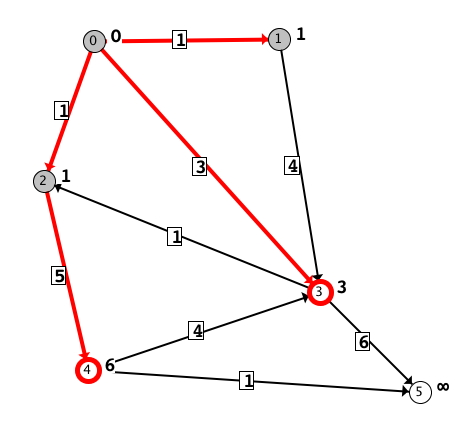
\includegraphics[scale=0.55]{X_dijkstra_directed}
\end{center}

\caption{Dijkstra's algorithm on a directed graph.}
\label{fig:dijkstra_directed}
\end{figure}


\begin{figure}[p]

\begin{center}
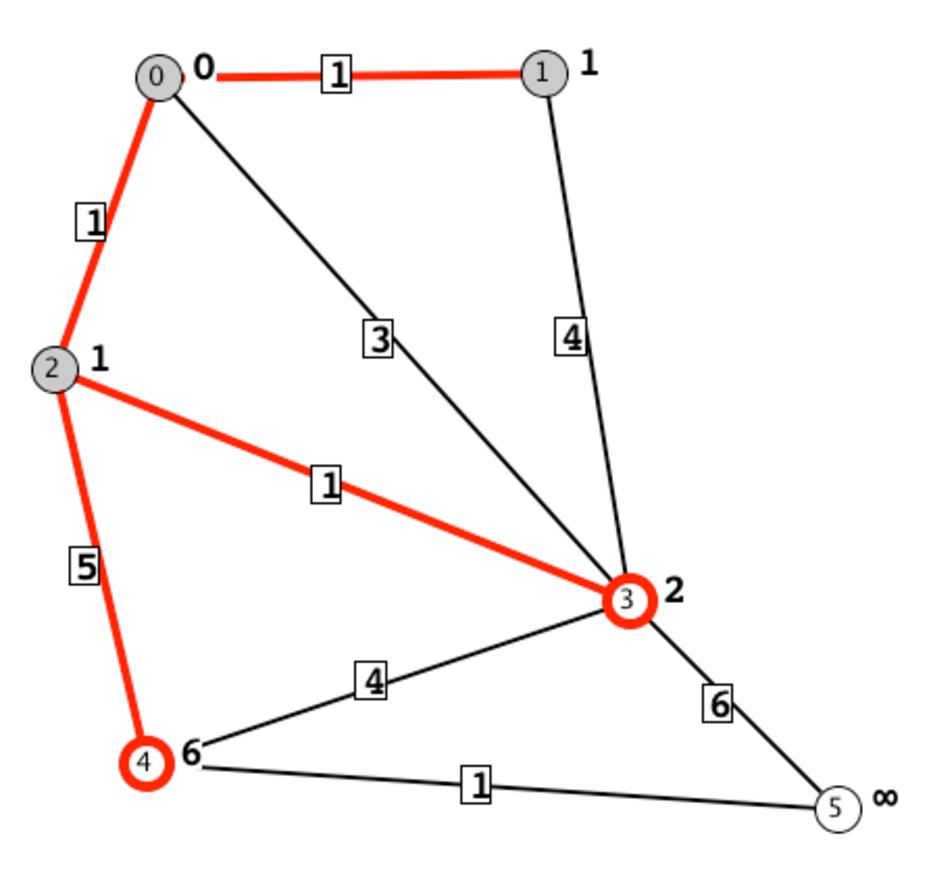
\includegraphics[scale=0.55]{X_dijkstra_undirected}
\end{center}

\caption{Dijkstra's algorithm on the same graph, undirected.}
\label{fig:dijkstra_undirected}
\end{figure}


The macro \emph{for\_outgoing($v,e,w$)}
creates a loop whose body is executed once
for each edge leading out of $v$; in the body, $e$ refers to the current edge
and $w$ to the other endpoint (any other variable names can be used).
In an undirected graph the term \emph{outgoing} applies to all incident
edges.\footnote{
Also provided are \emph{for\_incoming} and \emph{for\_adjacent};
the latter applies to all incident edges, even for directed graphs.
}

The difference between what the algorithm does on a directed versus an undirected graph is evident in the figures.
The edge \emph{from} node~3 to node~2 in the directed graph becomes an
edge \emph{between} the two nodes in the undirected form of the same graph.
Thus, in the undirected version, when node~2 is added to the tree
it also causes the distance from the source, node~0, to node~3 to be updated,
via the path through node~2.
These snapshots come from the executions of the \emph{same algorithm} on the
\emph{same graph}.
The only difference is that the explorer toggled from the directed to
the undirected
interpretation of the graph.

The array \verb+chosenEdge+ is required in order to control the highlighting.
Galant provides for seamless indexing of arrays with node id's: the
function \verb+nodeIds+ simply returns the largest node id plus one
(so that an array can be allocated correctly) and \verb+id(v)+ returns the
id of v, to be used as an index.
Node ids, therefore, need not be contiguous starting at 0, as,
in general, they won't be because of deletions or when graphs
come from external sources.


\subsection{Kruskal's algorithm}

\begin{figure}

{\small
\begin{verbatim}
// standard disjoint set untilities; not doing union by rank or path
// compression; efficiency is not an issue

Node [] parent;

function INIT_SET(Node x) { parent[id(x)] = x; }

function LINK(Node x, Node y) { parent[id(x)] = y; }

function Node FIND_SET(Node x) {
    if (x != parent[id(x)])
        parent[id(x)] = FIND_SET(parent[id(x)]);
    return parent[id(x)];
}

function UNION(Node x, Node y) { LINK(FIND_SET(x), FIND_SET(y)); }

algorithm {
    parent= new Node[nodeIds()];
    for_nodes(u) {
        INIT_SET(u);
    }

    EdgeList edgeList = getEdges();
    sort(edgeList);

    // MST is only relevant for undirected graphs
    setDirected(false);

    int totalWeight = 0;
    for ( Edge e: edgeList ) {
        beginStep();
        Node h = source(e);
        Node t = target(e);
        // show e's endpoints as it's being considered
        // marking is used for display purposes only
        mark(h); mark(t);
        endStep();

        beginStep();
        // if the vertices aren't part of the same set
        if ( FIND_SET(h) != FIND_SET(t) ) {
            // add the edge to the MST and highlight it
            highlight(e);
            UNION(h, t);
            totalWeight += e.getWeight();
            display( "Weight so far is " + totalWeight );
        }
        else {
            display( "Vertices are already in the same component." );
        }
        endStep();

        beginStep(); unMark(h); unMark(t); endStep();
    }
    display( "MST has total weight " + totalWeight );
}
\end{verbatim}
} % small

\caption{The implementation of Kruskal's algorithm animation.}
\label{fig:kruskals_algorithm}
\end{figure}


\begin{figure}[p]

\begin{center}
\fbox{
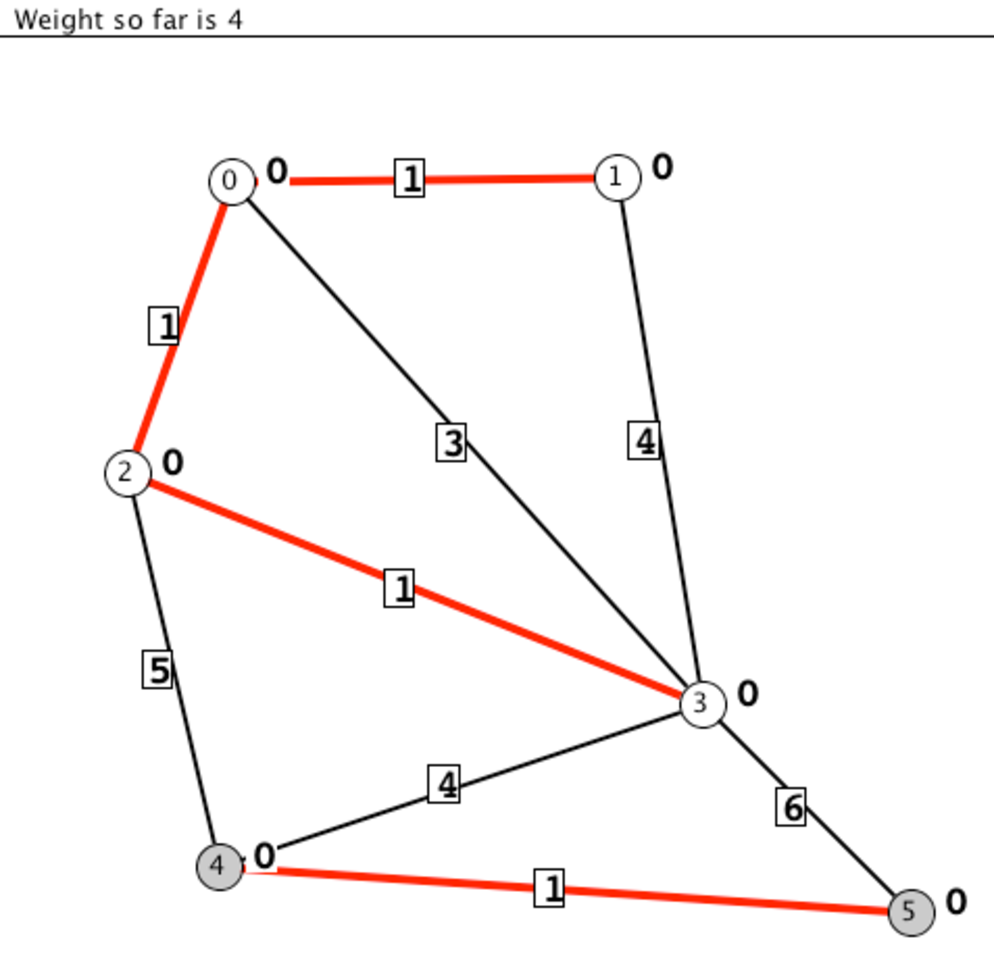
\includegraphics[scale=0.55]{X_kruskal_1}
}

(a) An edge is added to the tree.

\fbox{
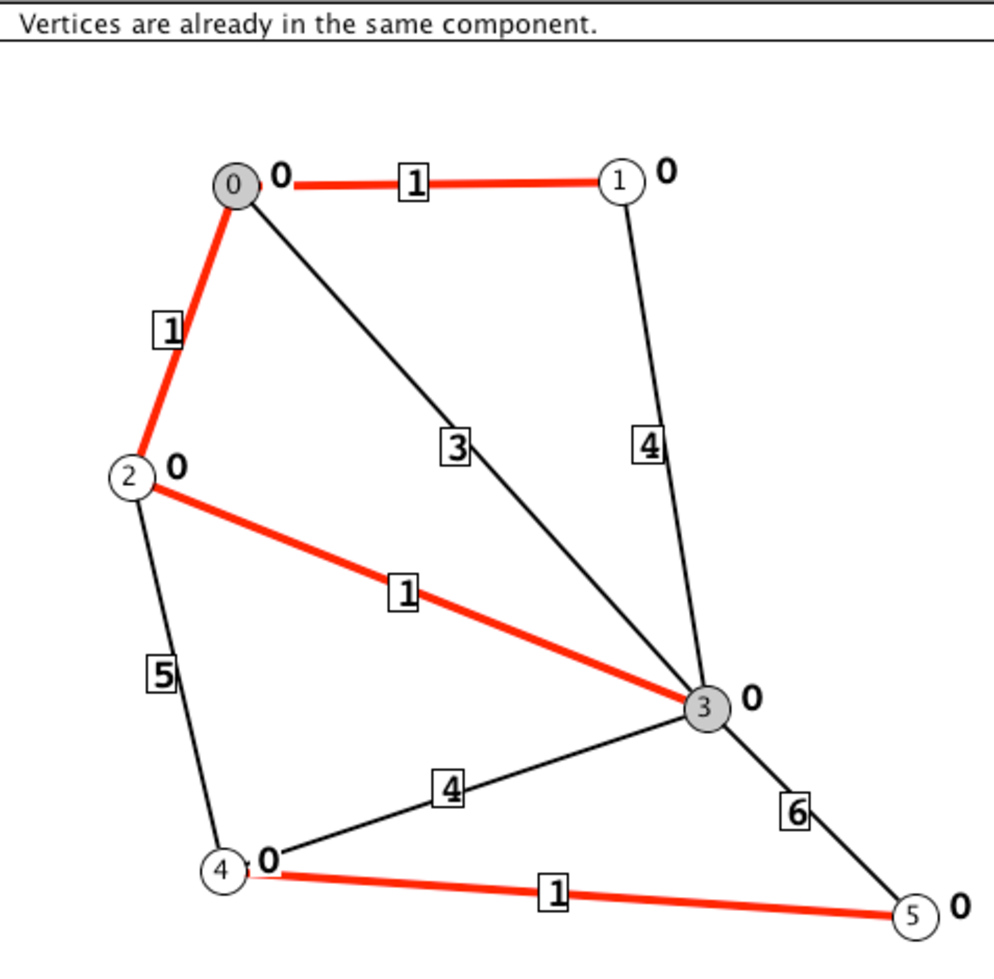
\includegraphics[scale=0.55]{X_kruskal_2}
}

(b) The current edge creates a cycle.

\end{center}

\caption{Two steps in Kruskal's algorithm. A message at the top left of the window describes the state of the algorithm.}

\label{fig:kruskal_pictures}
\end{figure}


Another simple algorithm implementation is that of Kruskal's algorithm
for finding a minimum spanning tree (or forest) in a graph.
Fig.~\ref{fig:kruskals_algorithm}
shows the implemented animation of Kruskal's algorithm.
Additional Galant features/workarounds illustrated here are:
\begin{itemize}

\item
Use of the keyword \verb+function+ to declare a function: this avoids the
syntactic complications of Java method declarations. In the case of
\verb+FIND_SET+, for example, you would normally have to say\\
\verb+static Node FIND_SET( Node x )+\\
and would get error messages about non-static methods in a static context
if you omitted the keyword \verb+static+.

\item
Implicit use of weights to sort the edges: weights are created by the
explorer when editing a graph. The only (syntactic) drawback is the required
use of the Java \verb+Collections.sort()+ construct, but this will be easy to fix in future releases.
Another piece of awkward syntax is the template invocation
\verb+List<Edge>+; again, this is easily fixable.

\item
The ability to write messages during execution, as accomplished by the
\verb+writeMessage+ calls.
The syntax that requires \verb+writeMessage+ to be a method of the \verb+Graph+
class is awkward, but can be remedied by augmenting the macro translation
mechanism.

\item
Declaration of a global array: the current implementation of Galant does
not provide a less Java-specific variant.
With moderate effort the Galant preprocessor could be augmented to provide
a more transparent syntax, such as\\
\verb+Node array parent[Node]+\\
The underlying implementation could either be a map (associative array) or an
array with integer indices but with nodes automatically converted to their
id's so that a reference to an element would always be \verb+parent[x]+
rather than \verb+parent[x.getId()]+.
In this specific situation -- implementation of disjoint set union --
the need for the array can be obviated by providing disjoint sets as
a built-in data structure.

\end{itemize}

Two steps in the execution of the animation are shown
in Fig.~\ref{fig:kruskal_pictures}.
The two endpoints of an edge are marked when that edge is considered
for inclusion in the spanning tree.
If the endpoints are not in the same tree, the edge is added and highlighted
and the cost of the current tree is displayed in the message.
Otherwise the message reports that the endpoints are already in the same tree. 


\subsection{Depth-first search (directed graphs)}


\begin{figure}

\begin{minipage}{0.5\textwidth}
\small
\begin{verbatim}
function visit( Node v ) {
  globals.time++;
  discovery[ v.getId() ] = globals.time;
  beginStep();
  v.setLabel( "" + discovery[ v.getId() ] );
  v.selected( true );
  endStep();
  for_outgoing( v, e, w ) {
    beginStep();
    if ( ! w.isSelected() ) {
      e.setSelected(true);
       visit( w );
    }
    else if ( finish[ w.getId() ] == 0 ) {
      e.setLabel( "B" );  /* ancestor */
    }
    else if ( finish[ w.getId() ]
              > discovery[ v.getId() ] ) {
      e.setLabel( "F" );  /* descendant */
    }
    else {
      e.setLabel( "C" );
    }
    endStep();
  }
  beginStep();
  globals.time++;
  finish[ v.getId() ] = globals.time;
  v.mark();
  v.setLabel( "" + discovery[ v.getId() ]
              + "/" + finish[ v.getId() ] );
  endStep();
}

setDirected( true );

beginStep();
for_nodes( u ) {
    u.setLabel("");
}
for_edges( e ) {
    e.setLabel("");
}
endStep();

for_nodes( u ) {
    if ( ! u.isSelected() ) {
        visit( u, null );
    }
}

\end{verbatim}
\end{minipage}
\begin{minipage}{0.49\textwidth}
\centering

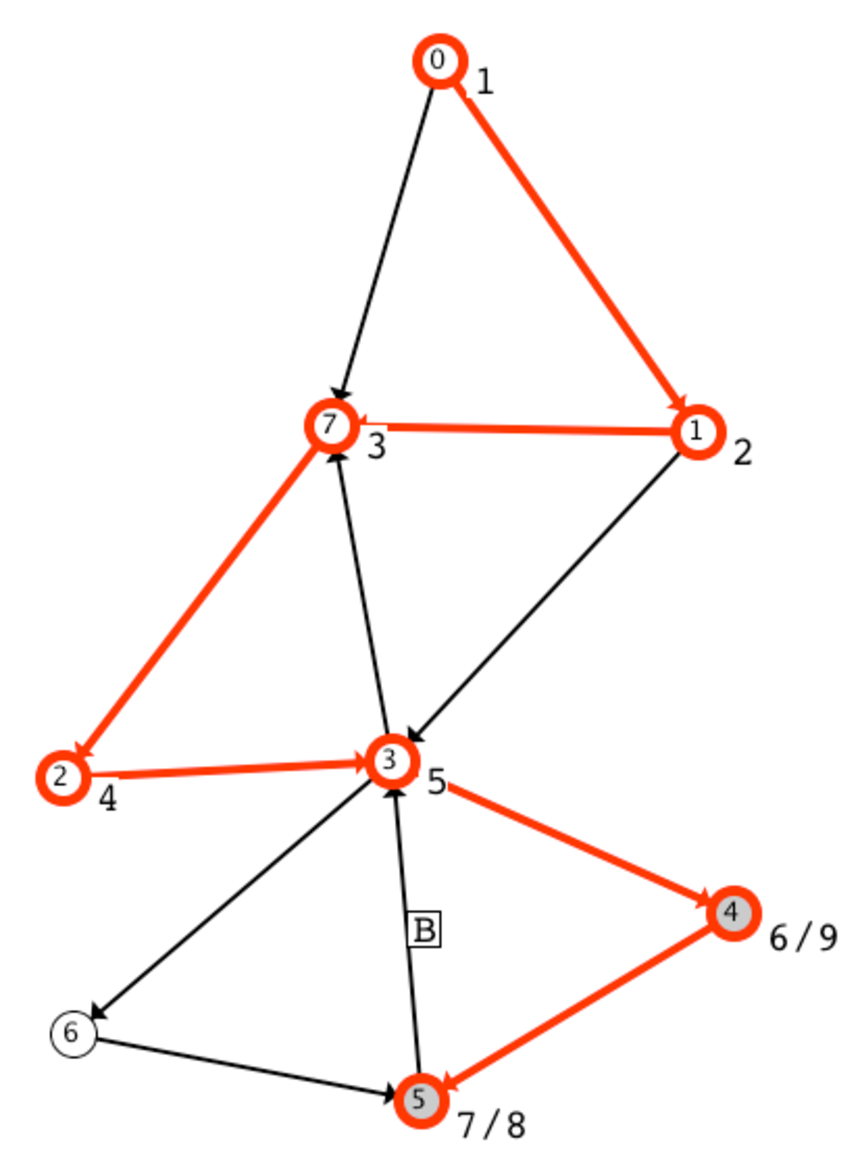
\includegraphics[scale=0.5]{X_dfs_d_1}

After first non-tree edge is labeled. 

\medskip

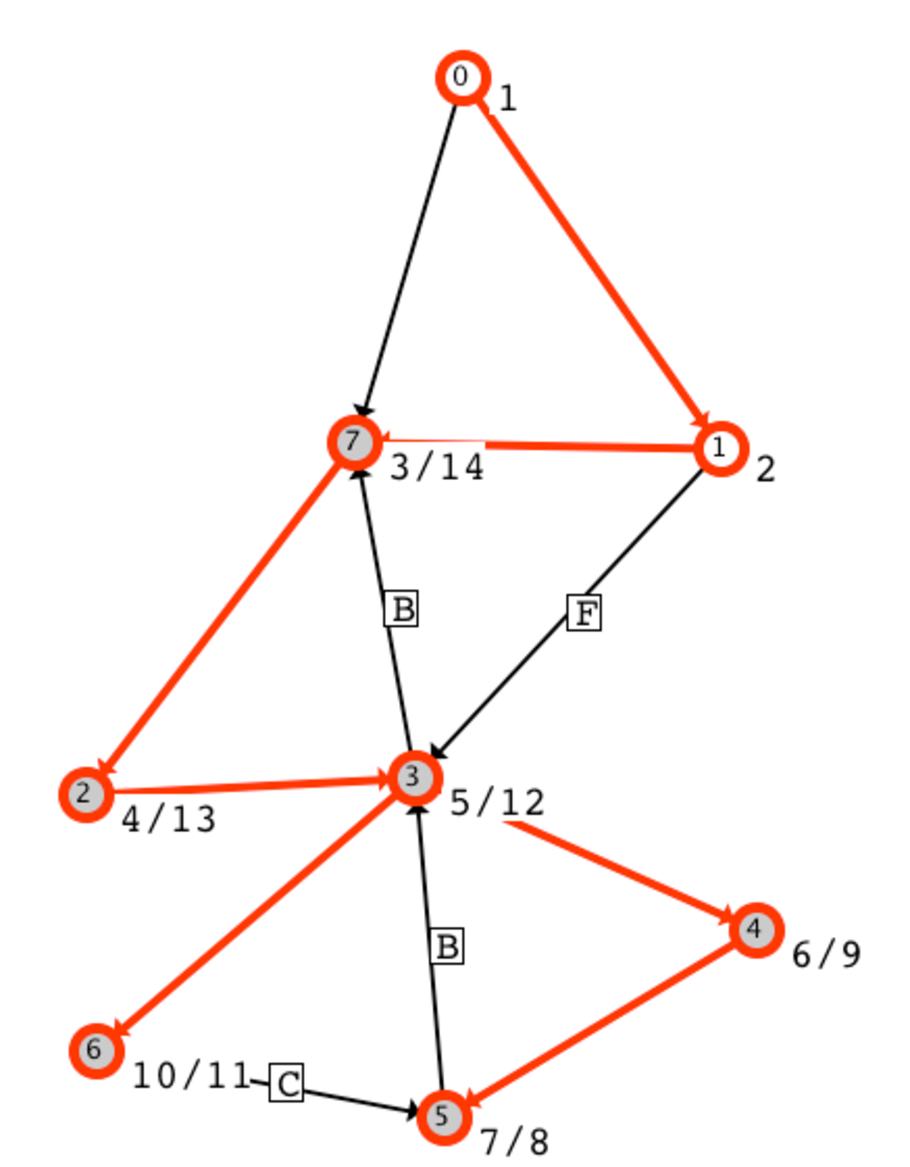
\includegraphics[scale=0.5]{X_dfs_d_2}

After all but one non-tree edges have been labeled.

\end{minipage}
\caption{Implementation of a depth-first search animation
  with an illustration of the graph panel during execution.}
\label{fig:dfs}
\end{figure}


Fig.~\ref{fig:dfs} illustrates an animation of depth-first search.
The code and definitions follow those of Cormen et al.~\cite{2009-Intro_to_Algorithms-Cormen}.
Tree edges are highlighted (selected)
and non-tree edges are labeled as \textbf{B}ack edges,
\textbf{F}orward edges or \textbf{C}ross edges.
White nodes, not yet visited,
are neither highlighted (selected) nor marked;
Gray nodes, visited but the visit is not finished, are highlighted only;
and black nodes, visit is completed, are both highlighted and 
marked.
Labels on nodes indicate the discovery and finish times, separated by a slash.

This particular algorithm, unlike our implementation of Dijkstra's,
is intended for a directed graph.
We would
need to write a different algorithm/animation
for undirected graphs.
When a graph is undirected an
edge is effectively directed both ways;
hence
tree
edges would get relabeled as back edges when they are encountered the second time.
The usual trick is to either mark edges if they have already been visited
or to keep track of the parent of a node when it is visited.


\subsection{Insertion sort}


\begin{figure}

\begin{center}

\begin{minipage}{4in}
\begin{verbatim}
    movesNodes();
    for ( int i = 1; i < numNodes; i++ ) {
        beginStep();
        Double x = A[i]; setWeight(toInsert, A[i]);
        setX(toInsert, xCoord[i]);
        endStep();
        Integer j = i - 1;
        while ( j >= 0 ) {  
            beginStep();
            setX(toInsert, xCoord[j]);
            highlight(nodes[j]);
            endStep();
            if ( A[j] <= x ) break;
            beginStep();
            A[j+1] = A[j]; setWeight(nodes[j+1], A[j]);
            unhighlight(nodes[j]);
            unmark(nodes[j]);
            mark(nodes[j+1]);
            endStep();
            j = j - 1;
        }
        beginStep();
        A[j+1] = x; setWeight(nodes[j+1], x);
        mark(nodes[j+1]);
        endStep();
    }
\end{verbatim}
\end{minipage}

% {\ttfamily
% \begin{alg}{4.0in}
% for ( int i = 1; i < n; i++ ) \{ \+\\
%     double x = A[i]; toInsert.setWeight( A[i] ); \\
%     toInsert.setX( xCoord[i] ); \\
%     endStep(); \\
%     int j = i - 1; \\
%     while ( j >= 0 \&\& A[j] > x ) \{ \+\\  
%         beginStep(); \\
%         toInsert.setX( xCoord[j] ); \\
%         highlight(nodes[j]); \\
%         endStep(); beginStep(); \\
%         A[j+1] = A[j]; nodes[j+1].setWeight( A[j] ); \\
%         nodes[j].unMark(); \\
%         nodes[j].setSelected( false ); \\
%         nodes[j+1].mark(); \\
%         endStep(); \\
%         j = j - 1; \-\\
%     \} \\
%     beginStep(); \\
%     A[j+1] = x; nodes[j+1].setWeight( x ); \\
%     nodes[j+1].mark(); \-\\
% \}
% \end{alg}
% } % ttfamily
% } % fbox

\bigskip

\fbox{
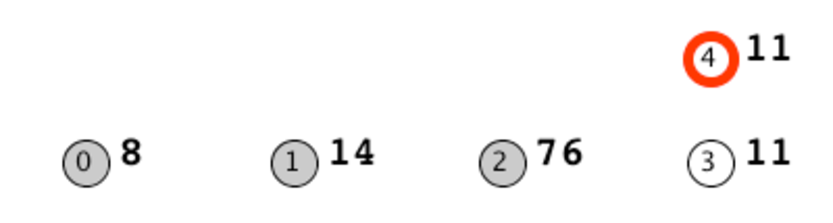
\includegraphics[scale=0.4]{X_is_1}
}

\smallskip
(a) Starting to insert \verb$x = A[3]$.

\bigskip
\fbox{
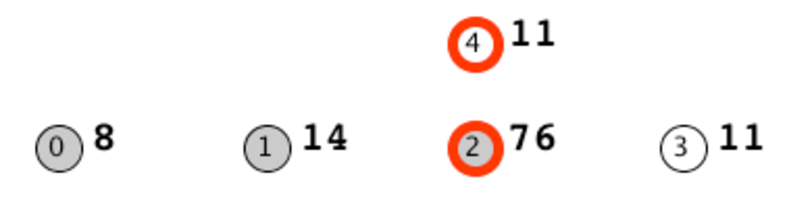
\includegraphics[scale=0.4]{X_is_2}
}

\smallskip
(b) Comparing \verb$x$ with \verb$A[2]$.

\bigskip
\fbox{
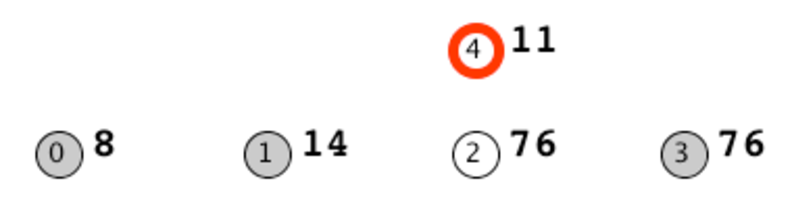
\includegraphics[scale=0.4]{X_is_3}
}

\smallskip
(c) \verb$A[2] > x$ so \verb$A[3] = A[2]$.

\end{center}

\caption{The insertion sort algorithm
and three steps in the animation.}
\label{fig:insertion_sort_animation}
\end{figure}


Fig.~\ref{fig:insertion_sort_animation}
illustrates an animation of insertion sort
that uses node movement and suggests that, with some creativity,
other sorting algorithms might be animated as well
-- this has already been done for bubble sort.
At the beginning (not shown) the code:
(i)~puts nodes, evenly spaced, on a horizontal line;
(ii)~creates arrays \verb$nodes$, \verb$xCoord$ and \verb$A$, holding the
nodes, their horizontal positions and their weights (i.e., the array to be sorted), respectively; and (iii)~adds a new node \verb$toInsert$ for the
element to be inserted at each outer-loop iteration.
The rest of the code is a classic insertion sort implementation: nodes behave
as if they were array positions; those in the already sorted part of the array
are marked; a node that is being compared with \verb$x$ is highlighted (selected).





\section{User documentation}
\label{sec:user_documentation}

What follows are instructions for interacting with the Galant GUI interface.

\subsection{Overview}

Galant provides three major components across two windows:
\begin{enumerate}
\item
a text window that can serve two distinct purposes --
\begin{enumerate}
\item as an editor of algorithms
\item as an editor of GraphML representations of graphs
\end{enumerate}
\item
a graph window that displays the current graph (independent of whether
the text window shows an algorithm or the GraphML representation of the graph)
\end{enumerate}

It is usually more convenient to edit algorithms
offline using a program editor.
The primary use of the text editor is to correct minor errors and
to see the syntax highlighting related to macros and Galant API functions.
The graph window is the primary mechanism for editing graphs.
One exception is when precise adjustments node positions are desired.
Weights and labels are sometimes also easier to edit in the text window.

\begin{figure*}
  \centering
    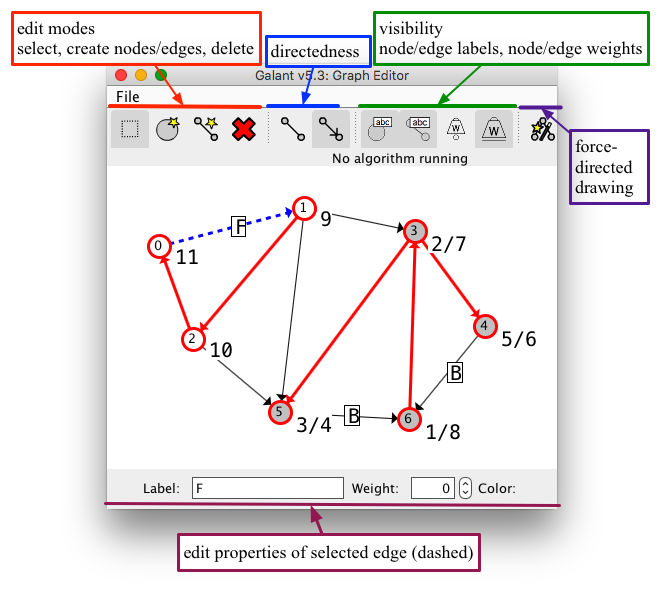
\includegraphics[scale=0.5]{X-graph_window-annotated}

    Graph window: add/delete nodes and edges, move nodes, etc.

    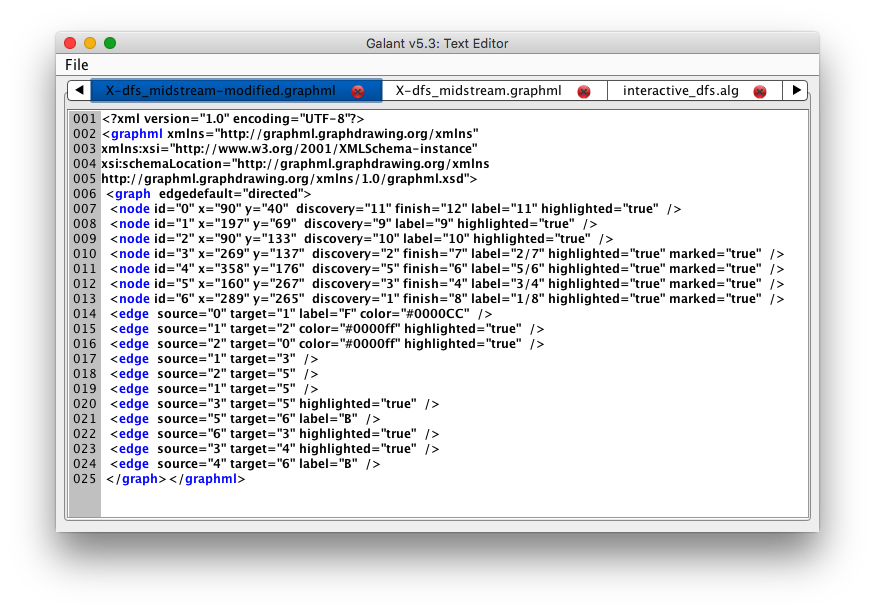
\includegraphics[scale=0.5]{X-dfs_midstream_modified-text}

    \vspace{-3ex}
    Text window: GraphML representation.

  \caption{The Galant user interface.}
  \label{fig:user_interface}
\end{figure*}

% [Last modified: 2016 12 13 at 21:24:38 GMT]


\begin{figure}[p!]
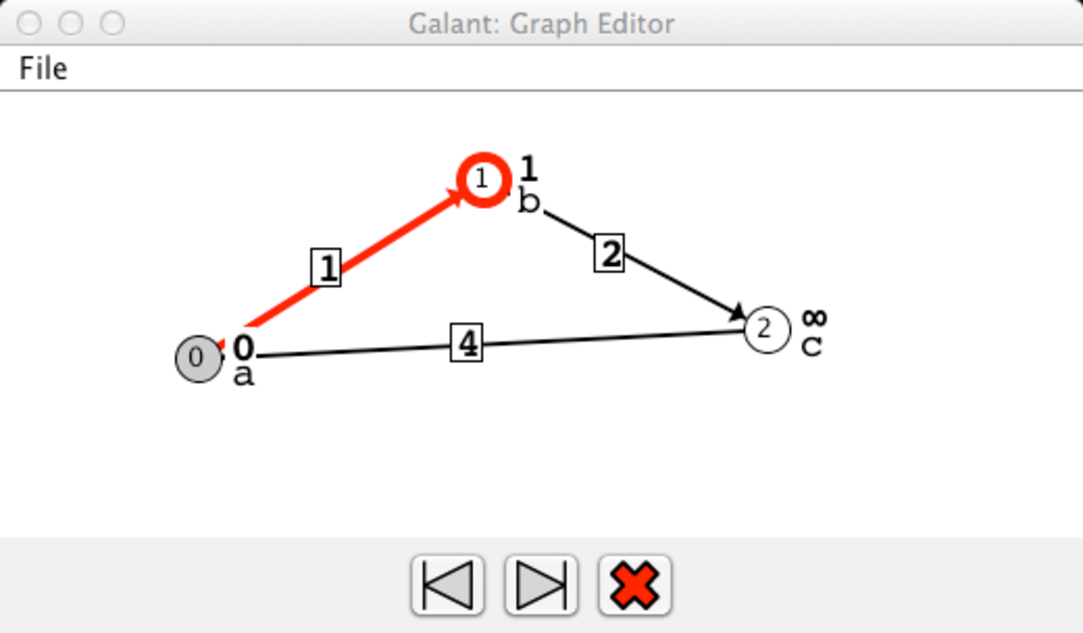
\includegraphics[scale=0.5]{X_dijkstra_running}
\caption{The graph window when Dijkstra's algorithm is running.}
\label{fig:dijkstra_running}
\end{figure}

These components operate in two modes: edit mode and animation mode.
Edit mode allows the user to modify graphs -- see Sec.~\ref{sec:graph_editing},
or algorithms -- see Sec.~\ref{sec:algorithm_editing}. Animation mode disables all forms of modification, allowing the user to progress through
an animation by stepping forward or backward, as described in
Sec.~\ref{sec:animating_algorithms}.

\subsection{Workspace}

Opened graph and algorithm files are displayed in the text window,
which has tabs that allow the user to switch among different algorithms/graphs.
New algorithms are created using the icon that looks like
a page of text at the top left of the
window; new graphs are created
using the graph/tree icon to the left of that.
More commonly, algorithm and graph files are loaded via the \Code{File->Open}
browser dialog. The \Code{File} drop-down menu also allows saving of files
and editing of preferences. Algorithm files have the extension \Code{.alg}
and graph files the extension \Code{.graphml}.

Fig.~\ref{fig:user_interface} shows both the graph window (top) and the text
window (bottom). Annotations on the graph window describe the components of
the window that can be used to edit a graph visually.

\subsection{Graph editing}
\label{sec:graph_editing}

Graphs can be edited in their GraphML representation using the text window
or visually using the graph window.
These editors are linked:
any change in the visual representation is immediately reflected in the text
representation (and will overwrite what was originally there);
a change in the GraphML representation will take effect in the visual representation
when the file is saved.

An improperly formatted GraphML file loaded from an external source will
result in an error.
Galant reports errors of all kinds (during reading of files, compilation of
animation programs or execution of animations)
by displaying a pop up window that allows the user to choose whether to
continue (and usually return to a stable state) or quit the program.
Error information, including a stack trace, is also displayed on the console.

The graph window, as illustrated at the top of Fig.~\ref{fig:user_interface},
has a toolbar with four sections:
\begin{enumerate}
\item
\textbf{Graph edit mode -- }
this includes the \emph{select}, \emph{create node}, \emph{create edge}, and \emph{delete} buttons.
Only one button is active at any time; it determines the effect
of a user's interaction (mouse clicking, dragging, etc.) with the window.
if there are conflicts in selection of objects, nodes with higher id numbers have precedence (are above those with lower id numbers) and nodes
have precedence over edges (are above edges).
\begin{itemize}
\item \emph{Select.} A mouse click selects the graph component with highest precedence.
If the component is a node, it is shaded light blue; if it's an edge, it
becomes dashed.
The in-line editor at the bottom of the graph window allows editing of the
component's label, weight, and color.
\item \emph{Create node.}
A node is created at the location of a mouse click if there is not already a node there.
If another node is present it is simply selected.
\item \emph{Create edge.}
Two clicks are required to create an edge. The first falls on the desired
source node and the second on the target node.
The line representing the edge is shown after the first click.
If the first click does not land on a node, no edge is created.
If the second click does not land on a node, creation of the edge is canceled.
\item \emph{Delete.}
A mouse click deletes the highest-precedence component at the mouse location.
If a node is deleted, all of its incident edges are deleted as well.
\end{itemize}

\item
\textbf{Directedness toggles --}
These change both the interpretation and the
display of the graph between directed and undirected.
Pressing the undirected (line without arrows) button causes
all edges to be interpreted as undirected: this means that, when the code
calls for all incoming/outgoing edges, all incident edges are used.
Undirected edges are displayed as simple lines.

Pressing the directed (line with arrow) button causes the macros
\Code{for\_incoming}, \Code{for\_outgoing}, and \Code{for\_adjacent}
to have three distinct meanings (they are all the same for undirected graphs):
Incoming edges have the given node as target, outgoing as source, and adjacent applies to all incident edges.

\item
\textbf{Display toggles --}
The four display toggles turn on/off the display of node/edge labels and node/edge weights.
A shaded toggle indicates that the corresponding display is \emph{on}.
When Galant is executed for the first time, all of these are \emph{on},
but their setting persists from session to session.
Labels and weights are also all displayed at the beginning of execution of
an animation.
The animation program can choose to hide labels and/or weights with simple
directives.
Hiding is usually unnecessary -- the graphs that are subjects of the animations
typically have only the desired attributes set.

\item
\textbf{Force directed drawing button -- }
Applies Hu's force directed algorithm~\cite{2006-Mathematica-Hu} to the graph.
Pushing the button a second time causes the drawing to revert to its previous state.

\end{enumerate}

Keyboard shortcuts for graph editing operations are as follows:

\begin{tabular}{l @{ -- } p{0.9\textwidth}}
\textsf{Ctrl-n} & create a new node in a random position \\
\textsf{Ctrl-e} & create a new edge; user is prompted for id's of the nodes to
be connected \\
\textsf{Ctrl-i} & do a smart repositioning (force-directed)
of nodes of the graph, useful when positions were chosen randomly;
when \Code{Ctrl-i} is used for smart repositioning (as
opposed to the toggle button, the user is prompted for a "degree repelling
boost", designed to prevent clustering of cliques or near-cliques in the
graph -- the higher the number, the more nodes of high degree will repel each
other (default is 3)
\\
\textsf{Del-n} & (hold delete key when typing \Code{n})
delete a node; user is prompted for id \\
\textsf{Del-e} & delete an edge; user is prompted for id's of the endpoints \\
\textsf{Ctrl-$\ell$} & toggle display of node labels \\
\textsf{Ctrl-L} & toggle display of edge labels \\
\textsf{Ctrl-w} & toggle display of node weights \\
\textsf{Ctrl-W} & toggle display of edge weights \\
\end{tabular}

\subsection{Algorithm editing}
\label{sec:algorithm_editing}

Algorithms can be edited in the text window. The
editor uses Java keyword highlighting (default blue) and
highlighting of Galant API fields and methods (default green).
Since the current algorithm editor is fairly primitive (no search and replace, for example),
it is more efficient to edit animation code offline using a program editor --
for example \Code{emacs} with Java mode turned on.
The Galant editor is, however, useful for locating and correcting minor errors.
For more details on how to compose animation code, see the programmer guide
(Section~\ref{sec:programmer_guide}).

\subsection{Animating algorithms}
\label{sec:animating_algorithms}

To animate an algorithm the code for it must be compiled and then run via the
algorithm controls
 -- the bottom tabs on the text window shown in Figs.~\ref{fig:algorithm_text}
and~\ref{fig:algorithm_running}.
The algorithm runs on the \emph{active graph}, the one currently displayed
on the graph window.
If there are errors in compilation these will show up on the console (terminal
from which Galant was run) and in a dialog box that allows the user to ask for more details
and decide whether to exit Galant or not.
The console also displays the what the code looks like after macro replacement
in case obscure errors were the result of unexpected macro expansion.
Line numbers in the macro-expanded code match those of the original so that
all errors reported by the Java compiler will refer to the correct line number
in the original Galant code.
Runtime errors also open the above mentioned
dialog box.

When the user initiates execution of an animation by pushing the \textsf{Run}
button
the animation program
steps forward until
displays the next animation event or, if a \Code{beginStep()}
call has marked the start of a sequence of events, until
it reaches the next \Code{endStep()} call.
It then pauses execution and waits for the user to decide whether to
step forward, step backward, or exit.
A step forward resumes execution while a step backward returns the display to a previous
state.
The algorithm resumes execution only when the \emph{display state}
indicated by the user's sequence of forward and backward steps
($f-b$, where $f$ is the number of forward and $b$ the number of backward steps)
exceeds the \emph{algorithm state}, the number of animation steps the algorithm
has executed.
The user controls forward and backward steps using either the buttons at the
bottom of the graph window (shown in Fig.~\ref{fig:dijkstra_running})
or the right/left arrow keys.
During the execution of the animation, all graph editing functions are disabled.
These are re-enabled when the user exits the animation by pressing the red \textbf{X} button or the \textsf{Esc} (escape) key on the terminal.

\subsection{Preferences}
\label{sec:preferences}

Galant preferences can be accessed via the \Code{File->Preferences}
menu item or by using the keyboard shortcut \textsf{Ctrl-P}
(\textsf{Cmd-P} for Mac).
Preferences that can be edited are:
\begin{itemize}
\item
Default directories for opening and saving files (\Code{Open/Save}).
\item
Directory where compiled animation code is stored (\Code{Compilation}).
\item
Font size and tab size for text window editing (\Code{Editors}).
\item
Colors for keyword and Galant API highlighting (\Code{Algorithm~Editor}).
\item
Color for GraphML highlighting (\Code{Textual~Graph~Editor}).
\item
Node radius (\Code{Graph~Display});
when the radius is below a threshold (9 pixels), node id's are not displayed;
this is useful when running animations on large graphs.
\item
Edge width (\Code{Graph~Display}).
\end{itemize}


% [Last modified: 2016 12 20 at 22:53:27 GMT]


\section{Programmer guide}
\label{sec:programmer_guide}
Animation programmers can write algorithms in notation that resembles
textbook pseudocode
in files that have a \Code{.alg} extension.
The animation examples have used procedural syntax for function calls, as in, for example,
\Code{setWeight(v,0)}.
Java (object oriented) syntax can also be used: \Code{v.setWeight(0)}.
A key advantage of Galant is that a seasoned Java programmer can
not only use the Java syntax but can also augment Galant algorithms with
arbitrary Java classes defined externally, using \Code{import} statements.
All Galant code is effectively Java, either natively, or via macro preprocessing.

The text panel provides a crude editor for algorithms (as well as GraphML
descriptions of graphs);
its limited capabilities make it useful primarily for fine tuning and error correction.
The animator should use a program editor such as \Code{Emacs} or
\Code{Notepad++} (in Java mode) to edit algorithms offline,
not a major inconvenience -- it is easy to reload algorithms when they are modified
without exiting Galant.
The Galant editor is, however, useful in that it provides syntax highlighting of Galant
functions and macros.

The source code for an algorithm begins with any number (including none)
of global variable declarations and function definitions.
The animator can import code from other sources using appropriate
\Code{import} statements; these must occur at the very beginning.
The code for the algorithm itself follows, starting with the keyword
\textsf{algorithm}.
A \emph{code block}
is a sequence of statements, each terminated by a semicolon, just as in
Java.
An animation program has the form
\begin{quote}
  \emph{global variable declarations}\\
  \\
  \emph{function definitions}\\
  \\
  \Code{algorithm \{}\\
  \hspace*{2em}\emph{code block}\\
  \Code{\}}
\end{quote}

Declarations of global variables are also like those of Java:\\
\hspace*{1em}\emph{type} \emph{variable\_name}\texttt{;}\\
or\\
\hspace*{1em}\emph{type} \texttt{[]} \emph{variable\_name}\texttt{;}\\
to declare an array of the given type.
All variables must be initialized either within a function definition or
in the algorithm.
Unlike Java variables, they cannot be initialized in the statement that
declares them.\footnote{This restriction applies to global variables
  only. Variables local to function definitions or to the algorithm can be
  initialized in-line, just as in Java.
}
The Java incantation\\
\hspace*{1em}\emph{type} \emph{variable\_name}
\texttt{= new} \emph{type}\texttt{[} \emph{size} \texttt{]}\\
is used to initialize an array with \emph{size} elements initialized to \textsf{null}
or 0.
Arrays use 0-based indexing: the largest index is $\mathit{size} - 1$.
Detailed
information about function declarations is in Section~\ref{sec:functions}
below.

Central to the Galant API is the \Code{Graph} object: currently all other
parts of the API refer to it.
The components of a graph are declared to be of type \Code{Node} or
\Code{Edge} and can be accessed/modified via a variety of
functions/methods.
When an observer or explorer interacts with the animation they move either
forward or backward one step at a time.
All aspects of the graph API therefore refer to the current \emph{state of
  the graph}, the set of states behaving as a stack.
API calls that change the state of a node or an edge automatically
generate a next step,
but the programmer can override this using a \Code{beginStep()} and
\Code{endStep()} pair. For example, the beginning of our implementation of
Dijkstra's algorithm looks like

\begin{center}
\begin{minipage}{0.5\textwidth}
\begin{verbatim}
beginStep();
for_nodes(node) {
    setWeight(node, INFINITY);
    nodePQ.add(node);
}
endStep();
\end{verbatim}
\end{minipage}
\end{center}

Without the \Code{beginStep}/\Code{endStep}
override, this initialization would require the observer to click
through multiple steps (one for each node) before getting to the interesting
part of the animation.
For convenience the function \Code{step()} is a synomym for \Code{endStep();~beginStep()}.
If a step takes longer than \Timeout\ seconds, the program is terminated
under the presumption that there may be an infinite loop.

\begin{table}
  \small
  \centering
  \begin{tabular}{| m{0.35\textwidth} | m{0.6\textwidth} |}
    \hline
    \shortstack[l]{
      \textsf{List$\langle$Node$\rangle$ getNodes()}\\
      \textsf{NodeList getNodes()}
    }
    &
    returns a list of the nodes of the graph; type \textsf{NodeList}
    is built into Galant
    and essentially equivalent to the Java \textsf{List$\langle$Node$\rangle$};
    see Table~\ref{tab:data_structures}
    \\ \hline
    \shortstack[l]{
      \textsf{List$\langle$Edge$\rangle$ edges()}\\
      \textsf{EdgeList edges()}
    }
    &
    returns a list of edges of the graph; return type
    \textsf{EdgeList} is analogous to \textsf{NodeList}
    \\ \hline
    \textsf{for\_nodes(v) \{
      \emph{statement; \ldots}
      \}}
    &
    \shortstack[l]{
      equivalent to
      \textsf{for ( Node v : nodes() ) \{ \emph{statement; \ldots} \}};\\
      the statements are executed for each node \textsf{v}
    }
    \\ \hline
    \textsf{for\_edges(e)  \{ \emph{statement; \ldots} \}}
    &
    analogous to \textsf{for\_nodes}
    \\ \hline
    \textsf{Integer numberOfNodes()}
    &
    returns the number of nodes
    \\ \hline
    \textsf{Integer numberOfEdges()}
    &
    returns the number of edges
    \\ \hline
    \textsf{int~id(Node~v)}, \textsf{int~id(Edge e)}
    &
    returns the unique identifier of \textsf{v} or \textsf{e}
    \\ \hline
    \textsf{int~nodeIds()}, \textsf{int~edgeIds()}
    &
    returns the largest node/edge identifier plus one;
    useful when an array is to be indexed using node/edge identifiers,
    since these are not necessarily contiguous
    \\ \hline
    \textsf{source(Edge e)}, \textsf{target(Edge e)}
    &
    returns the source/target of edge \textsf{e}, sometimes called the (arrow)
    tail/head or source/destination
    \\ \hline
    \shortstack[l]{
      \textsf{Integer degree(Node v)}\\
      \textsf{Integer indegree(Node v)}\\
      \textsf{Integer outdegree(Node v)}
    }
    &
    the number of edges incident on \textsf{v}, total, incoming and outgoing;
    if the graph is undirected, the outdegree is the same as the degree
    \\ \hline
    \shortstack[l]{
      \textsf{EdgeList edges(Node v)}\\
      \textsf{EdgeList inEdges(Node v)}\\
      \textsf{EdgeList outEdges(Node v)}
    }
    &
    returns a list of \textsf{v}'s
    indicent, incoming or outgoing edges, respectively;
    outgoing edges are the same as incident edges if the graph is undirected 
    \\ \hline
    \shortstack[l]{
      \textsf{Node otherEnd(Edge e, Node v)}\\
      \textsf{Node otherEnd(Node v, Edge e)}
    }
    &
    returns the node opposite \textsf{v} on edge \textsf{e};
    if \textsf{v} is the source \textsf{otherEnd} returns the target and
    vice-versa
    \\ \hline
    \textsf{NodeList neighbors(Node v)}
    &
    returns a list of nodes adjacent to \textsf{v}
    \\ \hline
    \shortstack[l]{
      \textsf{for\_adjacent(v, e, w) \{ \emph{code block} \}} \\
      \textsf{for\_incoming(v, e, w) \{ \emph{code block} \}} \\ 
      \textsf{for\_outgoing(v, e, w) \{ \emph{code block} \}}
    }
    &
    \textsf{for\_adjacent} executes the code block for each edge \textsf{e}
    incident on \textsf{v}, where \textsf{w} is \textsf{otherEnd(e,v)};
    \textsf{v} must already be declared but \textsf{e} and \textsf{w} are
    declared by the macro;
    the other two are analogous for incoming and outgoing edges 
    \\ \hline
    \textsf{getStartNode()}
    &
    returns the first node in the list of nodes, typically the one with smallest id;
    used by algorithms that require a start node
    \\ \hline
    \textsf{isDirected()}
    &
    returns true if the graph is directed
    \\ \hline
    \textsf{setDirected(boolean directed)}
    &
    makes the graph directed or undirected depending on whether \texttt{directed}
    is true or false, respectively
    \\ \hline
    \shortstack[l]{
      \textsf{Node addNode()}\\
      \textsf{Node addNode(Integer x, Integer y)}
    }
    &
    returns a new node and adds it to the list of nodes;
    the id is the smallest integer not currently in use as an id;
    attributes such as weight, label and position are absent and must be set explicitly
    by appropriate method calls;
    the second version sets the position of the node at \textsf{(x,y)}
    \\ \hline
    \shortstack[l]{
      \textsf{addEdge(Node source, Node target)}\\
      \textsf{addEdge(int sourceId, int targetId)}
    }
    &
    adds an edge from the source to
    the target (source and target are interchangeable when graph is undirected);
    the second variation specifies id's of the nodes to be connected;
    as in the case of adding a node, the edge is added to the list of edges and
    its weight and label are absent
    \\ \hline
    \textsf{deleteNode(Node v)}
    &
    removes node \textsf{v} and its incident edges from the graph
    \\ \hline
    \textsf{deleteEdge(Edge e)}
    &
    removes edge \textsf{e} from the graph
    \\ \hline
  \end{tabular}
  \caption{Functions and macros that apply to the structure of a graph.}
  \label{tab:graph_functions}
\end{table}


\begin{table}
  \small
  \centering
  \begin{tabular}{| m{0.35\textwidth} | m{0.6\textwidth} |}
    \hline
    \textsf{print(String s)}
    &
    prints \texttt{s} on the console; useful for debugging
    \\ \hline
    \textsf{display(String s)}
    &
    writes the string \textsf{s} at the top of the window
    \\ \hline
    \textsf{String getMessage()}
    &
    returns the message currently displayed on the message banner
    \\ \hline
    \textsf{error(String s)}
    &
    prints \textsf{s} on the console with a stack trace; also displays
    \textsf{s} in popup window with an option to view the stack trace;
    the algorithm terminates and the user can choose whether to terminate
    Galant entirely or continue interacting
    \\ \hline
    \textsf{beginStep()},
    \textsf{endStep()}
    &
    any actions between a \textsf{beginStep()} and an \textsf{endStep()}
    take place atomically, i.e.,
    all in a single ``step forward'' action by the user
    \\ \hline
    \textsf{Node getNode(String message)}
    &
    pops up a window with the given message and prompts the user to enter the
    identifier of a node, which is returned;
    if no node with that id exists,
    an error popup is displayed and the user is prompted again
    \\ \hline
    \textsf{Node getEdge(String message)}
    &
    pops up a window with the given message and prompts the user to enter the
    identifiers of two nodes, the endpoints of an edge, which is returned;
    if either id has no corresponding node or the the two nodes are not connect
    by an edge (in the right direction if the graph is directed),
    an error popup is displayed and the user is prompted again
    \\ \hline
    \shortstack[l] {
      \textsf{String getString(String message)}\\
      \textsf{Integer getInteger(String message)}\\
      \textsf{Double getReal(String message)}
    }
    &
    analogous to \textsf{getNode} and \textsf{getEdge}; allow algorithm to engage
    in dialog with the user
    \\ \hline
    \shortstack[l] {
      \textsf{Integer integer(String s)}\\
      \textsf{Double real(String s)}
    }
    &
    performs conversion from a string to an integer/double; useful when parsing
    labels that represent numbers
    \\ \hline
    \textsf{windowWidth()}, \textsf{windowHeight()}
    &
    current width and height of the window, in case the algorithm wants to rescale
    the graph
    \\ \hline
  \end{tabular}
  \caption{Utility functions.}
  \label{tab:utility_functions}
\end{table}



Functions and macros for the graph as a whole are shown in Table~\ref{tab:graph_functions}, while Table~\ref{tab:utility_functions} lists some algorithm functions not related to any aspect of a graph.

\emph{\textbf{Note:} The functions/methods provided by Galant may have multiple synonyms for
convenience and backward compatibility. A full list of methods and functions
is given in \Code{Algorithm.java} in the subdirectory
\Code{src/edu/ncsu/csc/Galant/algorithm}.}

The nodes and edges, of type \textsf{Node} and \textsf{Edge}, respectively,
are subtypes/extensions of \textsf{GraphElement}.
Arbitrary attributes can be assigned to each graph element. In the GraphML file
these show up as, for example,\\
\hspace*{3em}
\textsf{
$<$node \emph{attribute\_1}="\emph{value\_1}" ... \emph{attribute\_k}="\emph{value\_k}" /$>$
}

Each node and edge has a unique integer id.
The id's are assigned consecutively as nodes/edges are created;
they may not be altered.
The id of a node or edge can be accessed via the \Code{id()} function.
Often, as is the case with the depth-first search algorithm, it makes sense to use
arrays indexed by node or edge id's.
Since graphs may be generated externally and/or have undergone deletions of nodes or
edges, the id's are not always contiguous.
The functions \Code{nodeIds()} and \Code{edgeIds()} return the size of an array
large enough to accommodate the appropriate id's as indexes. So code such as

\begin{minipage}{0.8\textwidth}
\begin{verbatim}
        Integer myArray[] = new Integer[nodeIds()];
        for_nodes(v) { myArray[id(v)] = 1; }
\end{verbatim}
\end{minipage}

is immune to array out of bounds errors.

\subsection{Node and edge methods}

Nodes and edges have `getters' and `setters' for
a variety of attributes, i.e.,
\\
\Code{set}$a$\Code{($\langle a's$ type$\rangle$ x)}
\\
and
\\
$\langle a's$ type$\rangle$ \Code{get}$a$\Code{()},
where $a$ is the name of an attribute such as
\Code{Color},
\Code{Label} or \Code{Weight}.
A more convenient way to access these standard attributes omits the prefix \Code{get}
and uses procedural syntax:
\Code{color(}$x$\Code{)} is a synonym for $x$\Code{.getColor()}, for example.
Procedural syntax for the setters is also available:
\Code{setColor(}$x$,$c$\Code{)} is a synonym for $x$.\Code{setColor(}$c$\Code{)}.
In the special cases of color and label it is possible to omit the \Code{set}
(since it reads naturally):
\Code{color($x$,$c$)} instead of
\Code{setColor($x$,$c$)};
and
\Code{label($x$,$c$)} instead of
\Code{setLabel($x$,$c$)}.

\subsubsection{Logical attributes: functions and macros}

\textbf{Nodes.} From a node's point of view we would like information about
 the adjacent nodes and incident edges.  The relevant \emph{methods} require
 the use of Java generics, but macros are provided to simplify graph API
 access. The macros (which are borrowed from their equivalents in GDR) are:

\begin{itemize}

\item
\Code{for\_adjacent(x, e, y)\{ \emph{code block} \}}
executes the statements in the code block for each edge incident on \verb$x$.
The statements can refer to \verb$x$, or \verb$e$, the current incident edge,
or \verb$y$, the other endpoint of \verb$e$.
The macro assumes that \Code{x} has already been declared as \Code{Node}
but \Code{e} and \Code{y} are declared automatically.

\item
\Code{for\_outgoing(Node x, Edge e, Node y)\{ \emph{code block} \}}\\
behaves like \Code{for\_adjacent} except that, when the graph is directed,
it iterates only over the edges whose source is \verb$x$ (it still iterates over all the edges when the graph is undirected). 

\item
\Code{for\_incoming(Node x, Edge e, Node y)\{ \emph{code block} \}}\\
behaves like \Code{for\_adjacent} except that, when the graph is directed,
it iterates only over the edges whose sink is \verb$x$ (it still iterates over all the edges when the graph is undirected). 

\end{itemize}

The actual API methods hiding behind these macros are (these are Node methods):

\begin{itemize}
\item
\Code{List$\langle$Edge$\rangle$~edges($v$)} returns a list of all edges
incident to $v$, both incoming and outgoing.
\item
\Code{List$\langle$Edge$\rangle$~outgoingEdges($v$)} returns a list of edges
directed away from $v$ (all incident edges if the graph is undirected).
\item
\Code{List$\langle$Edge$\rangle$~incomingEdges($v$)} returns a list of edges
directed toward $v$ (all incident edges if the graph is undirected).
\item
\Code{Node~otherEnd($e$, $v$)} returns the endpoint, other than $v$, of $e$.
\end{itemize}

The following are node functions with procedural syntax.

\begin{itemize}
\item \Code{degree(v)}, \Code{indegree(v)} and \Code{outdegree(v)} return the appropriate
integers.
\item \Code{otherEnd(v, e)}, where \Code{v} is a node and \Code{e} is an edge
returns node \Code{w} such that \Code{e} connects \Code{v} and \Code{w};
the programmer can also say \Code{otherEnd(e, v)} in case she forgets the order
of the arguments.
\item \Code{neighbors(v)} returns a list of the nodes adjacent to node \Code{v}.
\end{itemize}

\bigskip
\textbf{Edges.}
The logical attributes of an edge $e$ are its source and target (destination)
accessed using \Code{source($e$)} and \Code{target($e$)}, respectively.

\bigskip
\textbf{Graph Elements.}
Nodes and edges both have a mechanism for setting (and getting)
arbitrary attributes of type Integer, String, and Double.
the relevant methods are listed below.
Note that the type can be implicit for the setters -- the compiler can figure
that out, but needs to be explicit for the getters -- in Java, two methods
that differ only in their return type are indistinguishable.
In each case $g$ stands for a graph element (node or edge).
\begin{itemize}
  \item \Code{set($g$, String \emph{attribute}, $\langle \mathit{type} \rangle$ \emph{value})},
    where \emph{type} can be \Code{String}, \Code{Boolean}, \Code{Integer},
    or \Code{Double}.
  \item \Code{set($g$, String \emph{attribute})}; the attribute is assumed to
    be Boolean, the value is set to \Code{true}.
  \item \Code{String getString($g$, String \emph{attribute})}
  \item \Code{Boolean getBoolean($g$, String \emph{attribute})}
    \item \Code{Boolean is(String \emph{attribute})}, a synonym for
      \Code{getBoolean} 
  \item \Code{Integer getInteger($g$, String \emph{attribute})}
  \item \Code{Double getDouble($g$, String \emph{attribute})}
\end{itemize}
An object oriented syntax can also be used -- this is especially natural in
case of \Code{is}, as in \Code{v.is("inTree")} -- see \Code{boruvka} in the
\Code{Algorithms} directory.
These are useful when an algorithm requires arbitrary information to be
associated with nodes and/or edges.
The user-defined attributes may differ from one node or edge to the next.
For example, some nodes may have a \Code{depth} attribute while others do not.

\subsubsection{Geometric attributes}

Currently, the only geometric attributes are the positions of the
nodes. 
Unlike GDR, the edges in Galant
are all straight lines and the positions of their labels are fixed.
The relevant methods for nodes -- using procedural syntax -- are
\Code{int~getX(Node)}, \Code{int~getY(Node)}
and \Code{Point~getPosition(Node)}
for the getters. To set a position,
one should use\\
\hspace*{2em}\Code{setPosition(Node,Point)}\\
or\\
\hspace*{2em}\Code{setPosition(Node,int,int)}.\\
Once a node has an established position, it is possible to change
one coordinate at a time using \Code{setX(Node,int)} or \Code{setY(Node,int)}.
Object-oriented variants of all of these, e.g.,
\Code{v.setX(100)}, are also available.

The user is allowed to move nodes during algorithm execution
and the resulting positions persist after execution terminates.
Node position is the only attribute that can be "edited" at runtime.
For some animations, however, such as sorting,
the animation itself needs to move
nodes.
To avoid potential conflicts between position changes inflicted by the user
and those desired by the animation.
the function \Code{movesNodes()}, called at the beginning of an algorithm
will prevent the user from moving nodes.

\subsubsection{Display attributes} \label{sec:display_attributes}

Each node and edge has
both a (double) weight and a label.
The weight
is also a logical
attribute in that
it is used implicitly as a
key for
sorting and priority queues.
The label is simply text and may be interpreted however the programmer
chooses.
The conversion functions \Code{integer(String)}
and \Code{real(String)}
-- see Table~\ref{tab:utility_functions}
-- provide a convenient mechanism for treating labels as objects of class
\Code{Integer} or \Code{Double}, respectively.
The second argument of \Code{label} (or single argument of the
object-oriented \Code{setLabel})
is not the expected \Code{String}
but \Code{Object};
any type of object that has a Java \Code{toString} method will work
-- numbers have to be of type \Code{Integer} or \Code{Double}
rather than \Code{int} or \Code{double} since the latter are not objects
in Java.\footnote{
  Galant functions return objects, \Code{Integer} or \Code{Double}, when
  return values are numbers for this reason.
}
Thus, conversion between string labels and numbers works both ways.

Aside from the setters and getters: \Code{setWeight(double)},
\mbox{\Code{Double getWeight()}}, \Code{setLabel(Object)}
and \mbox{\Code{String getLabel()}}, the programmer can also
manipulate and test for the absence of weights/labels using
\Code{clearWeight()} and \Code{boolean~hasWeight()},
and the corresponding methods for labels.
The procedural variants in this case are
\begin{itemize}
  \item \Code{setWeight(Node,double)},
  \item \mbox{\Code{Double getWeight(Node)}} or the more natural
    \mbox{\Code{Double weight(Node)}},
   \item \Code{setLabel(Node,Object)} or the more natural
     \Code{label(Node,Object)},
   \item \Code{getLabel(Node)} or the more natural
     \mbox{\Code{String label(Node)}}
\end{itemize}

Nodes can either be plain, highlighted (selected), marked (visited) or both highlighted and
marked.
Being highlighted alters the
the boundary (color and thickness) of a node (as controlled by the
implementation), while being marked affects the fill color.
Edges can be plain or selected, with thickness and color modified in the
latter case.

The relevant methods are
(here \Code{Element} refers to either a \Code{Node} or an \Code{Edge}):
\begin{itemize}
\item \Code{highlight(Element)}, \Code{unhighlight(Element)}
  and \Code{Boolean~isHighlighted(Element)}
\item correspondingly, \Code{setSelected(true)}, \Code{setSelected(false)},
and \Code{boolean~isSelected()}
\item \Code{mark(Node)}, \Code{unmark(Node)}
  and \Code{Boolean~isMarked(Node)},
  equivalently \Code{Boolean~marked(Node)}.
\end{itemize}

\begin{table}
  \centering
  \begin{tabular}{{| l @{~=~} l |}}
    \hline
    \texttt{RED} & \texttt{"\#ff0000"} \\ \hline
    \texttt{BLUE} & \texttt{"\#00ff00"} \\ \hline
    \texttt{GREEN} & \texttt{"\#0000ff"} \\ \hline
    \texttt{YELLOW} & \texttt{"\#ffff00"} \\ \hline
    \texttt{MAGENTA} & \texttt{"\#ff00ff" } \\ \hline
    \texttt{CYAN} & \texttt{"\#00ffff"} \\ \hline
    \texttt{TEAL} & \texttt{"\#009999"} \\ \hline
    \texttt{VIOLET} & \texttt{"\#9900cc"} \\ \hline
    \texttt{ORANGE} & \texttt{"\#ff8000"} \\ \hline
    \texttt{GRAY} & \texttt{"\#808080"} \\ \hline
    \texttt{BLACK} & \texttt{"\#000000"} \\ \hline
    \texttt{WHITE} & \texttt{"\#ffffff"} \\ \hline
  \end{tabular}
  \caption{Predefined color constants.}
  \label{tab:colors}
\end{table}

Although the specific colors for displaying the outlines of nodes
or the lines representing edges are
predetermined for plain
and highlighted nodes/edges,
the animation implementation can modify these colors,
thus allowing for many different kinds of highlighting.
The \Code{getColor} and \Code{setColor} methods
and their procedural variants have \Code{String} arguments
in the RGB format \texttt{\#RRGGBB}; for example,
the string \texttt{\#0000ff} is blue.
Here, as in the case of label, \Code{color($g$)} and \Code{color($g$,$c$)}
can be used in place of \Code{getColor($g$)} and \Code{setColor($g$,$c$)},
respectively.
Galant defines several color constants for convenience -- 
these are listed in Table~\ref{tab:colors} -- so one can say, e.g.,
\Code{color($g$,TEAL)} instead of \Code{color($g$,"\#009999")}.

Note: In the graph display \emph{highlighting takes precedence over color};
if a node is highlighted, its color is ignored and the default highlight
color is used.

Special handling is required when any attribute is nonexistent or has a
\Code{null} value -- these two are equivalent.
When displayed in the graph window, nonexistent labels and weights simply do
not show up while nonexistent colors are rendered as thin black lines
(thickness determined by user preference).
In an animation program, however, nonexistent attributes are handled
differently.
\begin{itemize}
\item \Code{color()} returns null as expected
\item all functions returning Boolean values, such as \Code{highlighted()},
  \Code{marked()} and those for attributes defined by the animator, return
  \Code{false}
\item \Code{label()} returns an empty string; this ensures that it is always
  safe to use a label in an expression calling for a string
\item \Code{weight()} throws an exception; there is no obvious default
  weight; a program can test for the presence/absence of a weight using the
  \Code{hasWeight()} or \Code{hasNoWeight()} methods
\end{itemize}

Of the attributes listed above, weight, label, color and position can be
accessed and modified by the user as well as the program.
In all cases (of display attributes -- recall that node positions are an
exception), modifications during runtime are ephemeral
-- the graph returns to its original, pre-execution, state after running the
animation.
The user can save the mid-execution state of the graph:
select the \Code{Export} option on the file menu of the
\emph{graph} window.

\begin{table}
  \small
  \centering
  \begin{tabular}{| m{0.4\textwidth} | m{0.55\textwidth} |}
    \hline
    \textsf{id(\emph{element})}
    &
    returns the unique identifier of the node or edge
    \\ \hline
    \textsf{mark(Node v), unmark(Node v)}
    &
    shades the interior of a node or undoes that
    \\ \hline
    \textsf{Boolean marked(Node v)}
    &
    returns \textsf{true} if the node is marked
    \\ \hline
    \textsf{highlight(\emph{element}), unhighlight(\emph{element})}
    &
    makes the node or edge highlighted, i.e.,
    thickens the border or line and makes it red / undoes the highlighting
    \\ \hline
    \textsf{Boolean highlighted(\emph{element})}
    &
    returns \textsf{true} if the node or edge is highlighted
    \\ \hline
    \shortstack[l]{
      \textsf{select(\emph{element})}, \textsf{deselect(\emph{element})}\\
      \textsf{selected(\emph{element})}
    }
    &
    synonyms for \textsf{highlight}, \textsf{unhighlight} and \textsf{highlighted}
    \\ \hline
    &
    \\ \hline
    \textsf{boolean set(\emph{element}, String key, $\langle$\emph{type}$\rangle$ value)}
    &
    sets an arbitrary attribute, \textsf{key}, of the element to have a value of a given type, where
    the type is one of \textsf{Integer}, \textsf{Double}, \textsf{Boolean}
    or \textsf{String};
    in the special case of \textsf{Boolean} the third argument may be omitted
    and defaults to \textsf{true};
    so \textsf{set(v,"attr")} is equivalent to \textsf{set(v,"attr",true)};
    returns \textsf{true} if the element already has a value for the given attribute,
    \textsf{false} otherwise
    \\ \hline
    \shortstack[l]{
    \textsf{$\langle$\emph{type}$\rangle$ get$\langle$\emph{type}$\rangle$(\emph{element}, String key)}\\
    \textsf{Boolean is(\emph{element}, String key)}
    }
    &
    returns the value associated with \textsf{key} or \textsf{null}
    if the graph has no value of the given type for \textsf{key}, i.e.,
    if no
    \textsf{set(String~key,~$\langle$\emph{type}$\rangle$~value)} has occurred;
    in the special case of a \textsf{Boolean} attribute, the second formulation
    may be used;
    the object-oriented syntax, such as \textsf{e.is("inTree")}, sometimes
    reads more naturally
    \\ \hline
  \end{tabular}

  \caption{Functions that query and manipulate attributes of individual
    nodes and edges.
    Here, \emph{element} refers to either a \textsf{Node} or an \textsf{Edge},
    both the type and the formal parameter.
  }
  \label{tab:graph_element_functions}
\end{table}


A summary of functions relevant to node and edge attributes (their procedural versions)
is given in Table~\ref{tab:graph_element_functions}.

\subsubsection{Global access for individual node/edge attributes and graph attributes}

\begin{table}
\centering

\small
\parbox{0.9\textwidth}{
  These functions are designed to access or manipulate attributes for all nodes or edges
  at once instead of individually.
  Also included are functions that deal with graph attributes.
}

\medskip
  \begin{tabular}{| m{0.37\textwidth} | m{0.58\textwidth} |}
    \hline
    \shortstack[l]{
      \Code{Boolean nodeLabelsAreVisible()}\\
      \Code{Boolean edgeLabelsAreVisible()}\\
      \Code{Boolean nodeWeightsAreVisible()}\\
      \Code{Boolean edgeWeightsAreVisible()}
    }
    &
    returns \Code{true} if node/edge labels/weights are \emph{globally} visible,
    the default state, which can be altered by \Code{hideNodeLabels()}, etc.,
    defined below
    \\ \hline
    \shortstack[l]{
      \Code{hideNodeLabels(), hideEdgeLabels()}\\
      \Code{hideNodeWeights(), hideEdgeWeights()}
    }
    &
    hides all node/edge labels/weights; typically used at the beginning of an algorithm
    to hide unnecessary information; labels and weights are shown by default
    \\ \hline
    \shortstack[l]{
      \Code{showNodeLabels(), showEdgeLabels()}\\
      \Code{showNodeWeights(), showEdgeWeights()}
    }
    &
    undoes the hiding of labels/weights
    \\ \hline
    \shortstack[l]{
      \Code{hideAllNodeLabels()}\\
      \Code{hideAllEdgeLabels()}\\
      \Code{hideAllNodeWeights()}\\
      \Code{hideAllEdgeWeights()}
    }
    &
    hides all node/edge labels/weights even if they are visible globally
    by default or by
    \Code{showNodeLabels()}, etc., or for individual nodes and edges;
    in order for the label or weight of a node/edge to be displayed,
    labels/weights must be visible globally and its label/weight must be visible;
    initially, all labels/weights are visible, both globally and for individual
    nodes/edges;
    these functions are used to hide information so that it can be revealed subsequently,
    one node or edge at a time
    \\ \hline
    \shortstack[l]{
      \Code{showAllNodeLabels()}\\
      \Code{showAllEdgeLabels()}\\
      \Code{showAllNodeWeights()}\\
      \Code{showAllEdgeWeights()}
    }
    &
    makes all individual
    node/edge weights/labels visible if they are globally visible by default
    or via \Code{showNodeLabels()}, etc.;
    this undoes the effect of \Code{hideAllNodeLabels()}, etc., and of
    any individual hiding of labels/weights
    \\ \hline
    \shortstack[l]{
      \Code{clearNodeLabels(), clearEdgeLabels()}\\
      \Code{clearNodeWeights(), clearEdgeWeights()}
    }
    &
    gets rid of all node/edge labels/weights; this not only makes them invisible,
    but also erases whatever values they have
    \\ \hline
    \Code{showNodes(), showEdges()}
    &
    undo any hiding of nodes/edges that has taken place during the algorithm
    \\ \hline
    \shortstack[l]{
      \Code{NodeSet visibleNodes()} \\
      \Code{EdgeSet visibleEdges()}
      }
    &
    return the set of nodes/edges that are not hidden
    \\ \hline
    \shortstack[l]{
      \Code{clearNodeMarks()}\\
      \Code{clearNodeHighlighting()}\\
      \Code{clearEdgeHighlighting()}
    }
    &
    unmarks all nodes, unhighlights all nodes/edges, respectively
    \\ \hline
    \shortstack[l]{
      \Code{clearNodeLabels()}\\
      \Code{clearNodeWeights()}\\
      \Code{clearEdgeLabels()}\\
      \Code{clearEdgeWeights()}
    }
    &
    erases labels/weights of all nodes/edges; useful if an algorithm needs to
    start with a clean slate with respect to any of these attributes
    \\ \hline
    \shortstack[l]{
      \Code{clearAllNode(String attribute)}\\
      \Code{clearAllEdge(String attribute)}
    }
    &
    erases values of the given attribute from all nodes/edges, a generalization of
    \Code{clearNodeLabels}, etc.
    \\ \hline
    \Code{boolean set(String attribute, $\langle$\emph{type}$\rangle$ value)}
    &
    sets an arbitrary attribute of the graph to have a value of a given type, where
    the type is one of \Code{Integer}, \Code{Double}, \Code{Boolean}
    or \Code{String};
    in the special case of \Code{Boolean} the second argument may be omitted
    and defaults to \Code{true};
    so \Code{set("attr")} is equivalent to \Code{set("attr",true)};
    returns \Code{true} if the graph already has a value for the given attribute,
    \Code{false} otherwise
    \\ \hline
    \shortstack[l]{
    \Code{$\langle$\emph{type}$\rangle$ get$\langle$\emph{type}$\rangle$(String attribute)}\\
    \Code{Boolean is(String attribute)}
    }
    &
    returns the value associated with \Code{attribute} or \Code{null}
    if the graph has no value of the given type for \Code{attribute}, i.e.,
    if no
    \Code{set(String~attribute,~$\langle$\emph{type}$\rangle$~value)} has occurred;
    in the special case of a \Code{Boolean} attribute, the second formulation
    may be used
    \\ \hline
    \shortstack[l]{
      \Code{clearAllNode(String attribute)}\\
      \Code{clearAllEdge(String attribute)}
    }
    &
    erases the value of the given attribute for all nodes/edges
    \\ \hline
  \end{tabular}

  \caption{Functions that query and manipulate graph
    node and edge attributes globally.}
  \label{tab:graph_attribute_functions}
\end{table}

% [Last modified: 2017 01 17 at 18:39:12 GMT]


It is sometimes useful to access or manipulate attributes of nodes and edges
globally.
For example, an algorithm might want to hide node weights entirely
because they are not relevant
or hide them initially and reveal them for individual nodes as
the algorithm progresses.
These functionalities can be accomplished by
\textsf{hideNodeWeights} or \textsf{hideAllNodeWeights}, respectively.
A summary of these capabilities is given in Table~\ref{tab:graph_attribute_functions}.

\subsection{Definition of Functions/Methods}\label{sec:functions}

A programmer can define arbitrary functions (methods) using the construct

\Code{function} \textsl{[return\_type]} \textsl{name} \Code{(}
 \textsl{parameters} \Code{) \{} \\
 \hspace*{3em} \emph{code block} \\
 \Code{\}}

The behavior is like that of a Java method. So, for example,
\begin{verbatim}
function int plus( int a, int b ) {
    return a + b;
}
\end{verbatim}
is equivalent to
\begin{verbatim}
static int plus( int a, int b ) {
    return a + b;
}
\end{verbatim}

The \textsl{return\_type} is optional. If it is missing, the function behaves like
a \textsf{void} method in Java. An example is the recursive function
\Code{visit} in depth-first search.
\\
\Code{function visit( Node v ) \{} \textsl{code} \Code{\}}

\begin{table}
  \small
  \centering

  \textbf{NodeList and EdgeList:} lists of nodes or edges, respectively.
  
  \medskip
  \begin{tabular}{| m{0.35\textwidth} | m{0.6\textwidth} |}
    \hline
    \shortstack[l]{
      \textsf{Node first(NodeList L)}\\
      \textsf{Edge first(EdgeList L)}
    }
    &
    returns the first element of this list
    \\ \hline
    \shortstack[l]{
      \textsf{add(Node v, NodeList L)}\\
      \textsf{add(Edge e, EdgeList L)}
    }
    &
    adds the node/edge to the end of the list \textsf{L}; along with \textsf{first}
    we get the effect of a queue
    \\ \hline
    \shortstack[l]{
      \textsf{remove(Node v, NodeList L)}\\
      \textsf{remove(Edge e, EdgeList L)}
    }
    &
    removes the first occurrence of node \textsf{v} or edge \textsf{e} from \textsf{L}
    \\ \hline
    \textsf{sort(NodeList L)}, \textsf{sort(EdgeList L)}
    &
    use the weights of the nodes/edges to sort the list \textsf{L}
    \\ \hline
  \end{tabular}  
  
\bigskip
  \textbf{NodeQueue and EdgeQueue:} queues of nodes or edges, respectively.

  \medskip
  \begin{tabular}{| m{0.35\textwidth} | m{0.6\textwidth} |}
    \hline
    \shortstack[l]{
      \textsf{void~enqueue(Node~v)},\\
      \textsf{void~enqueue(Edge~e)}
    }
    &
    adds \textsf{v} or \textsf{e} to the rear of the queue
    \\ \hline
    \textsf{Node~dequeue()}, \textsf{Edge~dequeue()}
    &
    returns and removes the \textsf{Node} or \textsf{Edge} at the front of the queue;
    returns \textsf{null} if the queue is empty
    \\ \hline
    \textsf{Node~remove()}, \textsf{Edge~remove()}
    &
    returns and removes the \textsf{Node} or \textsf{Edge} at the front of the queue;
    throws an exception if the queue is empty
    \\ \hline
    \textsf{Node~element()}, \textsf{Edge~element()}
    &
    returns the \textsf{Node} or \textsf{Edge} at the front of the queue
    without removing it;
    throws an exception if the queue is empty
    \\ \hline
    \textsf{Node~peek()}, \textsf{Edge~peek()}
    &
    returns the \textsf{Node} or \textsf{Edge} at the front of the queue
    without removing it;
    returns \textsf{null} if the queue is empty
    \\ \hline
    \textsf{size()}
    &
    returns the number of elements in the queue
    \\ \hline
    \textsf{isEmpty()}
    &
    returns \textsf{true} if the queue is empty 
    \\ \hline
  \end{tabular}

  \bigskip
  \textbf{NodeStack and EdgeStack:} stacks of nodes or edges, respectively.

  \medskip
  \begin{tabular}{| m{0.35\textwidth} | m{0.6\textwidth} |}
    \hline
    \shortstack[l]{
      \textsf{void~push(Node~v)},\\
      \textsf{void~push(Edge~e)}
    }
    &
    adds \textsf{v} or \textsf{e} to the top of the stack
    \\ \hline
    \textsf{Node~pop()}, \textsf{Edge~pop()}
    &
    returns and removes the \textsf{Node} or \textsf{Edge} at the top of the stack;
    throws an exception if the stack is empty
    \\ \hline
    \textsf{Node~peek()}, \textsf{Edge~peek()}
    &
    returns the \textsf{Node} or \textsf{Edge} at the top of the stack
    without removing it;
    returns null if the stack is empty
    \\ \hline
    \textsf{size()}, \textsf{isEmpty()}
    &
    analogous to the corresponding queue methods
    \\ \hline
  \end{tabular}

  \bigskip
  \textbf{NodePriorityQueue and EdgePriorityQueue:} priority queues of nodes or edges, respectively.

  \medskip
  \begin{tabular}{| m{0.35\textwidth} | m{0.6\textwidth} |}
    \hline
    \shortstack[l]{
      \textsf{void~add(Node~v)},\\
      \textsf{void~add(Edge~e)}
    }
    &
    adds \textsf{v} or \textsf{e} to the priority queue;
    the priority is defined to be its weight -- see Section~\ref{sec:display_attributes}
    \\ \hline
    \textsf{Node~removeMin()}, \textsf{Edge~removeMin()}
    &
    returns and removes the \textsf{Node} or \textsf{Edge} with minimum weight;
    returns \textsf{null} if the queue is empty
    \\ \hline
    \hline
    \shortstack[l]{
      \textsf{boolean~remove(Node~v)},\\
      \textsf{boolean~remove(Edge~e)}
    }
    &
    removes \textsf{v} or \textsf{e};
    returns \textsf{true} if the \textsf{v} or \textsf{e} is present,
    \textsf{false} otherwise
    \\ \hline
     \shortstack[l]{
      \textsf{void~decreaseKey(Node~v,~double~key)},\\
      \textsf{void~decreaseKay(Edge~e,~double~key)}
    }
    &
    changes the weight of \textsf{v} or \textsf{e} to the new key
    and reorganizes the priority queue appropriately;
    since this is accomplished by removing and reinserting the object, i.e.,
    inefficiently, this method can also be used to increase the key
    \\ \hline
    \textsf{size()}, \textsf{isEmpty()}
    &
    analogous to the corresponding queue methods
    \\ \hline
  \end{tabular}

  \caption{Built-in data structures and their methods.
     These methods use object-oriented syntax:
$\langle$\emph{structure}$\rangle$.$\langle$\emph{method}$\rangle$($\langle$\emph{arguments}$\rangle$)
    and are created using, e.g.,
    \textsf{NodeQueue~Q~=~new~NodeQueue();} the \textsf{new} operator in Java.
  }
  \label{tab:data_structures}
\end{table}


\subsection{Data Structures}

Galant provides some standard data structures for nodes and edges automatically.
These are described in detail in Tables~\ref{tab:algorithm_data_structures} and~\ref{tab:graph_data_structures}.
Table~\ref{tab:algorithm_data_structures} gives information about the simpler
structures -- lists, stacks and queues,
while Table~\ref{tab:graph_data_structures} describes the more sophisticated
-- sets and priority queues.

Data structures use object-oriented syntax.
For example, to add a node \Code{v} to a \Code{NodeList} \Code{L},
the appropriate syntax is \Code{L.add(v)}.
Most data structure operations are as efficient as one might expect.
A notable exception is \Code{decreaseKey}
for priority queues.
The operation \Code{pq.decreaseKey(v,k)}
does \Code{pq.remove(v)} followed by \Code{pq.add(v)}.
The new key is implicit -- it is the weight of the element.
In practice, assuming \Code{pq} is a \Code{NodePriorityQueue},
\Code{v} is a \Code{Node}
and \Code{k} is a \Code{Double}, the sequence would be
\begin{verbatim}
     setWeight(v, k);
     pq.decreaseKey(v,k);
\end{verbatim}
which would translate to
\begin{verbatim}
     setWeight(v, k);
     pq.remove(v);
     pq.add(v)
\end{verbatim}
As pointed out earlier,
the weight of a node or edge is used for priority in a priority
queue or for sorting.
The programmer can change this default
as well as the fact that the nodes/edges prioritized by increasing weight
(the priority queue is a min-heap).

The functionality of a priority queue depends on how it is initialized via a
constructor. Taking \Code{EdgePriorityQueue} as an example
(\Code{NodePriorityQueue} is analogous), the standard initialization, one
that defines a min-heap that uses weights as key is\\
\Code{EdgePriorityQueue q = new EdgePriorityQueue()}\\
or the
declaration\\
\Code{EdgePriorityQueue q}\\
could be separate from\\
\Code{q = new EdgePriorityQueue()}\\

Variations on the constructor call (part following \Code{new}) are
\begin{itemize}
\item \Code{EdgePriorityQueue(true)} to create a max-heap based on weights
  (if the argument is \Code{false} the result is a min-heap, the default)
\item \Code{EdgePriorityQueue("attribute")}, where \Code{"attribute"} is a
  numerical attribute of an edge
\item \Code{EdgePriorityQueue("attribute", true)} to create a max-heap with
  the given attribute.
\end{itemize}

\cmt{A workaround to the fact that the "attribute" constructors don't work is
a setAttribute() method}

\subsection{Queries}

An animation program can query the user for various kinds of input.
For example, the \Code{interactive\_dfs} algorithm asks the user to give a
starting node for a (directed) depth-first search and to give another start
node if the search terminates before all nodes are visited. The different
query options are listed in Table~\ref{tab:utility_functions}.

A query statement in an animation program initiates an algorithm step
unconditionally, i.e., even if it occurs within a
\Code{beginStep}-\Code{endStep} pair.
After the user responds to the query she has to do another step forward
before the animation proceeds (except in case of a Boolean query).
If the user steps backward after responding to a query, the query is not
invoked again. Subsequent forward steps use the same answer.
Thus it is not possible to allow a user to explore multiple alternative
executions in the same run (such a feature would require major enhancements
to the existing implementation).

Queries for nodes and edges ask for node id's (two of them in case of an
edge). Galant checks whether an id is that of a valid node and, in case of an
edge, whether an edge between the two nodes exists. If the graph is currently
directed, the direction of the edge also has to correspond. Any violation
causes an exception to be thrown -- a popup window reports the nature of the
error and allows the user to choose (a) different id(s).
The animator can impose additional restrictions by specifying a set of
permissible nodes/edges (unvisited nodes in the case of
\Code{interactive\_dfs}). If so, the animator also specifies an error message
in case the additional restriction is violated.

Other queries allow an animation to get strings, Boolean values, or numbers
from the user. Examples are in the \Code{binary\_tree} and \Code{grid}
algorithms which create complete binary trees or grid graphs based on tree
height or grid dimensions, respectively, specified as integers by the user.
These queries work the same way as those for vertices and edges. In case of
numbers Galant checks whether the input string is a valid integer or
floating point number and reports an error otherwise.

Boolean queries are a special case. The user does not type a response. The
only options are to press one of two buttons with the mouse or to press the
\Code{Enter} key to specify the default answer (true).
The animator can specify the text displayed on the buttons; defaults are
\Code{"yes"} and \Code{"no"}.
Another difference with Boolean queries is that the algorithm steps forward
immediately when the user responds to the query.\footnote{The reason this is
  not the case with other queries is that errors may need to be handled
  before the algorithm can proceed. Synchronization between the query and the
  algorithm is not straightforward.}

\subsection{Exceptions: Compile and Runtime Errors}

\begin{table}
  \small
  \centering
  \begin{tabular}{| p{0.3\textwidth} | c | p{0.5\textwidth}|}
    \hline
    \multicolumn{1}{|c|}{\textbf{message}}
    & \textbf{type/source}
    & \multicolumn{1}{c|}{\textbf{explanation}} \\
    \hline
    programmer message $m$ & runtime
    & animation program has encountered an \Code{error($m$)} call
    \\
    \hline
    programmer message $m$ & runtime
    & user selected a node or edge not in the set speficied by a query of the
    form \Code{getNode/getEdge($p$, $S$, $m$)}, where $p$ is the prompt, $S$
    the set, and $m$ the error message 
    \\
    \hline
    Nonexistent node or edge & runtime
    & a node/edge is null or does not exist in current state
    \\
    \hline
    Graph element has no weight & runtime
    & no weight was given, neither during editing nor earlier during execution
    \\
    \hline
    No edge with source $v$ and target $w$ exists & runtime
    & can occur when user responds to a query for an edge or the algorithm asks
    for a specific edge using \Code{getEdge($v,w$)}
    \\
    \hline
    Empty graph & runtime & animation attempts to get a node when there is
    none
    \\
    \hline
    No node with id $i$ exists & runtime
    & called \Code{getNodeById($i$)} when no node with id $i$ exists
    \\
    \hline
    Node has been deleted & runtime
    & called \Code{getNodeById($i$)} when node has been deleted
    \\
    \hline
    Attempt to removeMin from max heap (or vice versa) & runtime
    & priority queues can be initialized as either min heaps or max heaps;
    Galant checks to make sure the correct remove method is used
    \\
    \hline
    Attempt to add null node/edge to (priority) queue & runtime
    & what it says, prevents later problem with null element
    \\
    \hline
    Node/edge has no attribute $a$ when attempting to add to priority queue
    & runtime
    & Attribute $a$, which was specified as the one to use for comparisons
    when the priority queue was initialized, is not present for the element;
    the default attribute is \Code{weight}
    \\
    \hline
    Unable to compute center for node & any time
    & something got messed up with the x and y coordinates (or the layer
    information in case of a layered graph), e.g., with a \Code{setPosition}
    call
    \\
    \hline
    Something went wrong when processing algorithm block & macro processing
    & probably some unbalanced parens, braces or brackets in the algorithm
    \\
    \hline
    Missing \emph{right paren, bracket, brace} in \emph{code} \ldots
    & macro processing
    & what it says; the \emph{code} shows only the beginning of the code
    block in which the error occurred
    \\
    \hline
    \emph{macro name}: Curly braces required & macro processing
    & missing curly braces after a function header
    \\
    \hline
    No compiler found, need a JDK & compiler
    & either no JDK is installed or \Code{JAVA\_HOME} is not set up correctly
    \\
    \hline
    Invalid tab - use untitled graph or untitled algorithm & text editor
    & attempt to save a file when there's something wrong with the current
    tab/panel (should not happen)
    \\
    \hline
    No text when invoking GraphMLParser & GraphML parser
    & attempting to parse empty file
    \\
    \hline
    Missing id for node & GraphML parser
    & no id specified for the node; nodes are required to have id's; they are
    optional for edges
    \\
    \hline
    Bad id & GraphML parser
    & the id of a node or edge is not an integer
    \\
    \hline
    Duplicate id $i$ & GraphML parser
    & there is more than node/edge with id $i$
    \\
    \hline
    Missing source/target & GraphML parser
    & an edge has no source/target in its GraphML representation
    \\
    \hline
    Bad source/target id & GraphML parser
    & the source/target specified in the GraphML file is not a legal integer
    \\
    \hline
    Source/target node missing & GraphML parser
    & the integer id of the source/target does not correspond with any node
    \\
    \hline
    Bad weight & GraphML parser
    & the weight of a node/edge is not a valid floating point number
    \\
    \hline
    Bad x/y-coordinate & GraphML parser
    & the x or y coordinate of a node is not a legal integer
    \\
    \hline
    Missing/bad layer/positionInLayer & GraphML parser
    & something is wrong with layer or positionInLayer of a node in a layered
    graph
    \\
    \hline
  \end{tabular}

  \caption{Galant exceptions.}
  \label{tab:galant_exceptions}
\end{table}

% [Last modified: 2017 01 12 at 18:50:45 GMT]


Errors can occur at compile time, either because a macro is malformed or
because the Java code, after macro translation, has errors.
The reporting of Java compiler errors is straightforward. They are reported,
with line numbers, on the console. The line numbers correspond to those in
the Java code listing that also appears on the console (even if there are no
errors). In almost all cases the line numbers also correspond to those of the
original algorithm (before macro translation) in the text
window.\footnote{The only known exception is a function definition where the
  parameters are placed on multiple lines.}

Errors due to malformed macros are not, unfortunately, reported with line
numbers. To make matters worse, unbalanced parentheses or braces inside a
function definition or one of the \Code{for\_\ldots} macros result in a
malformed macro exception. The best strategy is to use a program editor that
does automatic indentation.

Runtime errors are also reported with (almost always correct) line
numbers. Galant makes every effort to catch errors before they result in, for
example, null pointer exceptions in the Galant implementation. Every function
with a graph element argument checks that the argument is not null and
reports a \Code{GalantException} if it is.
The second or third line in the stack trace
refers to the point in the algorithm where the exception occurred.
All exceptions, whether those caught as \Code{GalantException}'s with
meaningful messages or those caught in the Galant impemmentation code, result
in a stack trace on the console and a popup window.
The latter allows to user to choose whether to continue, meaning that the
algorithm is terminated and Galant returns to edit mode, or exit from Galant
completely.

Exceptions can also occur in edit mode: when reading a graph from a
file, when specifying a node or edge after a keyboard shortcut, or when
giving the weight of a node or edge.
A complete list of Galant exceptions is in Table~\ref{tab:galant_exceptions}.

% [Last modified: 2017 01 11 at 03:19:32 GMT]


\section{Known Bugs and Annoyances}
\label{sec:bugs}

\subsubsection*{Input/output}

\begin{itemize}

\item
When you save the current state of an animation using \texttt{File->Export}
on the graph panel some of the information might not be saved.
In particular, weights and labels are saved, but highlighting is not (since it is not equivalent to an actual color change of a node or edge).

\end{itemize}

\subsubsection*{Text editing (of programs or graphs)\footnote{
Galant's editor  is primitive, but
programs can easily be edited externally.
Text representations of graphs can either be edited or generated externally.}}

\begin{itemize}

\item
Tabs for graphs and algorithms are often hard to deal with: (a) if you reread
a graph or algorithm, it appears twice; (b) you can only run an algorithm on a graph if the tabs for the two appear at the top of the window at the same time
-- although the tabs bar can be ``scrolled'',
this may be impossible if there are other intervening graphs and algorithms.

\item If you attempt to do anything in the text window (File menu or tabs)
  while an algorithm is running, Galant hangs; it appears that you can quit it from
the file menu of the graph window, however.

\end{itemize}

\subsubsection*{Graph editing (in graph panel or via keyboard shortcuts)}

\begin{itemize}

\item
It is not possible to change the thickness of an edge or node boundary directly
from the editor or an algorithm nor is it possible to change the fill color of a node.
The only way to change these properties is via highlighting, selecting, and
marking nodes/edges during the animation.

\item
A change in color of an edge does not appear to take place while the edge
is selected for editing -- its color stays blue during that time.
Only when focus is no longer on the edge does it change color.

\item If user attempts to change weight/label of a node/edge and clicks on
  the graph panel in the middle of the operation, the change is lost. There
  is no ``ok'' prompt as with color.

\item When user creates a new edge via keyboard shortcut, there is no obvious
  way to enter the weight and label.

\end{itemize}

\subsubsection*{Compilation and execution}

\begin{itemize}

\item
The macro preprocessor is oblivious to comments. Thus, the placement or contents of a comment may cause it to throw an exception.
Such exceptions have been known to occur when comments appear inside functions
or contain constructions that are subject to macro expansion.
For example, sometimes the word \texttt{for} in a comment causes problems.

\item Every once in a while an exception occurs when an error-free algorithm
  is executed or when Galant intitally fires up, but it is possible to step
  through the animation normally after hitting the \textsf{Continue} button.

\item 
  The \texttt{function} construct appears not to work if the arguments or
  return value are arrays (or lists?).
  Macro expansion for this construct is complex.

\item
Compiler error messages can be cryptic (but at least they refer to the correct
line numbers). Because of the macro preprocessing, it may be necessary to look at the console to get an idea of what is causing a particular error.

\item
There is no way for the user to change anything about the display while stepping through the animation, such as, for example, changing visibility of labels and weights,
or positions of nodes to make important features more visible.

\item
There is no way for the animation program to specify that labels and/o weights
should be displayed or hidden.

\item
There is no way to execute the animation in a continuous fashion with a
controllable speed. The current workaround is the use of arrow keys as keyboard
shortcuts for stepping forward or backward -- these can be held down to
generate multiple steps in rapid succession, but the user must click on the
graph panel before starting the animation; for some reason, there is no
reaction to the shortcuts if the first mouse click is on one of the arrows at the bottom of the graph window.

\end{itemize}



\end{document}

% [Last modified: 2013 07 12 at 21:05:53 GMT]
